\documentclass[12pt]{article}

\usepackage{hcmus-report-template}

% Disable indentation on new paragraphs
\setlength{\parindent}{0pt}

% Line spacing 1.5
\renewcommand{\baselinestretch}{1.5}

% Optional: graphic path
% \graphicspath{PATH_TO_GRAPHIC_FOLDER}

% To use Times font family, uncomment this row
% \usepackage{mathptmx}

% To use roman section / subsection, uncomment these rows
% \renewcommand{\thesection}{\Roman{section}}
% \renewcommand{\thesubsection}{\thesection.\Roman{subsection}}

% Define course name, report name and report title.
\newcommand{\coursename}{Nhập môn lập trình kết nối vạn vật - 21KHDL}
\newcommand{\reportname}{Smart Lighting System (Phiên bản cải tiến)}
\newcommand{\reporttitle}{Báo cáo Đồ án cuối kỳ}

\newcommand{\studentname}{& Trần Hiếu Tâm (21127423)}
\newcommand{\teachername}{
& TS. Nguyễn Đức Hoàng Hạ & \\
& ThS. Đỗ Thị Thanh Hà & \\}


% Header
\lhead{\small\reporttitle\\Đề tài: \reportname}
\rhead{\small
Trường Đại học Khoa học Tự nhiên, ĐHQG-HCM\\
\coursename
}

% Footer
%\newcommand{\leftfooter}{Trần Hiếu Tâm (21127423)}
\lfoot{\leftfooter}

\usepackage{geometry}
\usepackage{array}
\usepackage{multirow}
\usepackage{longtable}  % Required for long tables that span multiple pages
\usepackage{verbatim}
\usepackage[utf8]{inputenc}
\usepackage{tikz} % Package for graphics

\usetikzlibrary{trees} % Import tree library for TikZ

\usepackage{dashrule}


\usepackage{xcolor}
\definecolor{titlepagecolor}{RGB}{0, 63, 136} % Light gray
\definecolor{titletextcolor}{RGB}{255, 255, 255}
\definecolor{customblue}{HTML}{335AFF}
\definecolor{customblue_old}{HTML}{243c74}


% ============ DOCUMENT ============
\begin{document}

\pagenumbering{roman}

% {\fontfamily{pcr}\selectfont}

\color{titletextcolor}
\pagecolor{titlepagecolor}

\newgeometry{left=3cm}
\begin{titlepage}


\begin{tikzpicture}[remember picture, overlay]
    \foreach \y in {0,...,8} { % Adjust range for number of stripes
        \fill[customblue] (current page.south west) ++(0, \y*0.45cm) rectangle ++(\paperwidth, 0.17cm); % Adjust thickness here
    }
\end{tikzpicture}


\newcommand{\HRule}{\rule{\linewidth}{0.5mm}}


\includegraphics[scale=.15]{img/Logo-FIT.png}\\[1cm] 
% \begin{tikzpicture}[remember picture, overlay]
%     % Image in the bottom-right corner behind text
%     \node[anchor=south east, opacity=0.9] at (current page.south east) {
%         
\includegraphics[width=8.5cm]{img/Picture1.png} % Adjust size as needed
%     };
% \end{tikzpicture}


{ 
\huge{\bfseries{\reporttitle}}\\[0.5cm]
% \Large{\bfseries\MakeUppercase{\reporttitle}}\\[0.5cm]
\large{\bfseries{Đề tài: \reportname}}
}\\[0.4cm]

\emph{Sinh viên thực hiện:}\\
\studentname\\[1cm]

\emph{Giảng viên hướng dẫn:} \\
\teachername\\[3cm]

{\large TP. Hồ Chí Minh, tháng 12 năm 2024}

\vfill


\end{titlepage}
	

\restoregeometry
\nopagecolor
\color{black}

% -------------------------------

\begin{titlepage}
\newcommand{\HRule}{\rule{\linewidth}{0.5mm}}


\centering


%\textsc{\Large đại học quốc gia tp. hồ chí minh}\\[0.5cm]
\normalsize{
\textsc{TRƯỜNG ĐẠI HỌC KHOA HỌC TỰ NHIÊN}\\
\textsc{\textbf{KHOA CÔNG NGHỆ THÔNG TIN}}\\[1.25cm]
}
%\textsc{bộ môn công nghệ tri thức}\\[0.5cm]

\includegraphics[scale=.1]{img/Logo-TA.png}\\[1cm] 


{ 
\huge{\bfseries{\reporttitle}}\\[0.5cm]
\large{\bfseries{Đề tài: \reportname}}
}\\[0.4cm]

\textbf{\large Học phần: \coursename}\\[2.5cm]

{\normalsize
\emph{Sinh viên thực hiện:}\\
\studentname
\vspace{0.4cm}

\emph{Giảng viên hướng dẫn:} \\
\teachername
}

% \begin{minipage}[t]{0.4\textwidth}
% \begin{flushleft} 
% \normalsize % Set text to normal size
% \emph{Sinh viên thực hiện:}\\
% \studentname
% \end{flushleft}
% \end{minipage}
% ~
% \begin{minipage}[t]{0.4\textwidth}
% \begin{flushright} 
% \normalsize % Set text to normal size
% \emph{Giảng viên hướng dẫn:} \\
% \teachername
% \end{flushright}
% \end{minipage}\\[4cm]

\vspace{4cm}

{\normalsize TP. Hồ Chí Minh, tháng 11 năm 2024}\\[3cm]


\vfill
\end{titlepage}


\begin{titlepage}
\setlength{\parindent}{1cm}
\newgeometry{left=4cm, right=4cm}

% \newcommand{\HRule}{\noindent\dotfill}
\newcommand{\HRule}{
    \begin{center}
        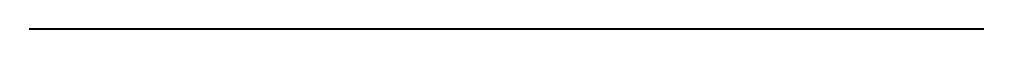
\begin{tikzpicture}
            \draw[thick, left color=gray, right color=white] (0,0) -- (\linewidth,0);
        \end{tikzpicture}
    \end{center}
}

\begin{center}
    \vspace*{1cm} % Use \vspace* for fixed positioning on the page
    {\Huge{\textbf{Lời mở đầu}}}    
\end{center}

\vspace{0.15cm} % Small space between title and line
\HRule % Minimalist thin line
\vspace{0.2cm} % Reduced space between line and content

Đồ án này là một phần của học phần \textit{Nhập môn lập trình kết nối vạn vật} - lớp 21KHDL, được tổ chức tại Khoa Công nghệ Thông tin, Trường Đại học Khoa học Tự nhiên, ĐHQG-HCM nhằm mục tiêu học tập, ứng dụng kiến thức IoT với tính chất là một đồ án phi thương mại. 


Em xin chân thành cảm ơn TS. Nguyễn Đức Hoàng Hạ, ThS. Đỗ Thị Thanh Hà, giảng viên Khoa Công nghệ Thông tin đã tận tình tư vấn, hỗ trợ về mặt kiến thức và định hướng, giúp cá nhân em hiểu rõ hơn về các nguyên lý và kỹ thuật cần thiết để hoàn thành đồ án này.
Đồng thời xin cảm ơn bạn Trần Lê Kim Ngân, sinh viên Khoa Điện tử Viễn thông, đã hỗ trợ nhiệt tình các linh kiện và vật liệu dựng mô hình cần thiết, góp phần quan trọng vào thành công của đồ án.


Sự hỗ trợ quý báu này là động lực quan trọng để bản thân em có thể hoàn thành dự án một cách tốt nhất. Mọi góp ý xin liên hệ qua email \href{mailto:thtam21@clc.fitus.edu.vn}{thtam21@clc.fitus.edu.vn}.\\[0.05cm]


\textit{Trân trọng,}


Trần Hiếu Tâm
\vspace{0.1cm} % Small space between title and line
\HRule % Minimalist thin line

\vfill

\end{titlepage}
\restoregeometry

\tableofcontents
\pagebreak
\listoftables
\pagebreak
\listoffigures
\pagebreak

\pagenumbering{arabic}
\setcounter{page}{1}


% \section{Section}

\subsection{Một số lưu ý}

\subsubsection{Cài đặt offline}
Template này yêu cầu cài đặt một số gói (package) nâng cao cho TexStudio:
\begin{itemize}
\item Để gõ thuật toán: \texttt{algorithm} và \texttt{algpseudocode}
\item Để nhúng (chèn) code: \texttt{listings}
\end{itemize}
Các gói này được cài đặt thông qua lệnh
\begin{lstlisting}[language=sh]
sudo apt-get install texlive-full
\end{lstlisting}
Tuy nhiên kích thước gói đâu đó vào khoảng 5GB (!). Vì vậy tốt nhất nên xài Overleaf.

\subsubsection{Sử dụng font khác}
Tham khảo font typefaces tại \href{https://www.overleaf.com/learn/latex/Font_typefaces}{link này}.

\subsubsection{Đánh số chỉ mục bằng chữ số La Mã}
Mở file \texttt{main.tex} và bỏ comment dòng 
\begin{lstlisting}[language=tex]
% \renewcommand{\thesection}{\Roman{section}}
% \renewcommand{\thesubsection}{\thesection.\Roman{subsection}}  
\end{lstlisting}

\subsection{Ví dụ}
Ngày xửa ngày xưa, ở vương quốc VNUHCM - US, có một chàng hoàng tử ngồi cắm đầu viết doc\footnote{Đây là footnote, chú thích lại những gì cần chú ý.}.\\
Mặc định muốn xuống dòng chỉ cần dùng $\backslash\backslash$  (2 lần dấu xẹt huyền).\\
Nếu bạn muốn thụt đầu dòng khi bắt đầu paragraph mới, vào \texttt{main.tex} và disble dòng
\begin{lstlisting}[language=tex]
\setlength{\parindent}{0pt}
\end{lstlisting}

\subsection{First subsection}
\subsubsection{First sub-subsection}
Subsection để ví dụ thôi. Thêm vài ví dụ:
\begin{itemize}
    \item Dùng itemize
    \item Vẫn là itemize
\end{itemize}
Sau đó xài enumerate:
\begin{enumerate}
    \item Dùng enumerate
    \item Vẫn là enumerate
\end{enumerate}
Nhỏ hơn subsubsection thì xài \texttt{paragraph}:

\paragraph{Đây là ví dụ cho paragraph}
Lưu ý là paragraph không nằm trong Mục lục.

\subsection{Chia nhỏ nội dung}
Bạn có thể chia nhỏ nội dung của báo cáo thành các file \texttt{.tex} và dùng lệnh \texttt{input} để chèn vào báo cáo chính. Ví dụ có trong file \texttt{main.tex}.
% \section{Hình ảnh}
Hình ảnh được thể hiện như hình~\ref{fig:my_label}, lưu ý flag \texttt{[H]} để disable floating (hình được hiển thị đúng vị trí, không trôi lên đầu trang).
\begin{figure}%[H]
\centering
\includegraphics[scale=.4]{img/hcmus-logo.png}
\caption{Hình ví dụ (logo HCMUS - updated 30/11/2022)}
\label{fig:my_label}
\end{figure}

Hình~\ref{fig:my_label_with_H} cũng là hình ví dụ nhưng có tag \texttt{[H]}. Lưu ý là có tag \texttt{[H]} thì code ở đâu hình sẽ nằm ở đó, không quan trọng nội dung ít hay nhiều (trang giấy sẽ thừa 1 khúc như bạn thấy). Để hiểu hơn về positioning trong LaTeX, xin tham khảo \href{https://www.overleaf.com/learn/latex/Positioning_images_and_tables}{bài này}.

\begin{figure}[H]
\centering
\includegraphics[scale=.4]{img/hcmus-logo.png}
\caption{Hình ví dụ (logo HCMUS - updated 30/11/2022)}
\label{fig:my_label_with_H}
\end{figure}
% \section{Bảng biểu}
Bảng biểu được thể hiện như bảng~\ref{tab:my_label}, lưu ý flag \texttt{[H]} để disable floating (bảng được hiển thị đúng vị trí, không trôi lên đầu trang). Bảng~\ref{tab:my_label} là một trường hợp không sử dụng tag \texttt{[H]} và bảng bị trôi tít lên đầu trang:
\begin{table}%[H]
\centering
\begin{tabular}{|l|l|}
\hline
\textbf{Tên con vật} & \textbf{Số chân} \\ \hline
Gà & 2 \\ \hline
Chó & 4 \\ \hline
Trần Hoàng Tử & 2 \\ \hline
\end{tabular}
\caption{Số chân của một số con vật, không có tag \texttt{[H]}}
\label{tab:my_label}
\end{table}

Bảng~\ref{tab:my_label_with_H_tag} thể hiện bảng biểu với tag \texttt{[H]}\footnote{Tương tự cách sử dụng tag \texttt{[H]} với hình}. Để không phải mất thời gian tuổi trẻ ngồi chỉnh table, xài \href{https://www.tablesgenerator.com}{https://www.tablesgenerator.com}.

\begin{table}[H]
\centering
\begin{tabular}{|l|l|}
\hline
\textbf{Tên con vật} & \textbf{Số chân} \\ \hline
Gà & 2 \\ \hline
Chó & 4 \\ \hline
Trần Hoàng Tử & 2 \\ \hline
\end{tabular}
\caption{Số chân của một số con vật, có tag \texttt{[H]}}
\label{tab:my_label_with_H_tag}
\end{table}.
% \section{Công thức toán}
Công thức toán gõ chung 1 dòng thì dùng 2 lần dấu dollar: $f(x) = x^2 + 2x + 1$. Với công thức nằm riêng 1 dòng thì gõ 2 cặp dấu dollar:
$$
ReLU(x) = \max(0, x)
$$
Siêu việt hơn, gõ hệ phương trình thì nên dùng tag \texttt{equation}
\begin{equation*}
\begin{aligned}
a_1x_1 + a_2x_2 + .. + a_nx_n &= u \\
b_1x_1 + b_2x_2 + .. + b_nx_n &= v \\
c_1x_1 + c_2x_2 + .. + c_nx_n &= w \\
\end{aligned}
\end{equation*}
Tham khảo cách gõ equation trên \href{https://www.overleaf.com/learn/latex/Mathematical_expressions}{Overleaf} nhé!
% \section{Thuật toán}
Dùng gói \texttt{algorithm} và \texttt{algpseudocode} để gõ đoạn thuật toán~\ref{alg:label}\footnote{Tất nhiên đây là dùng katana mổ ruồi!}

\begin{algorithm}
\caption{Thuật toán đếm xem nhiều gà hay nhiều chó hơn}
\label{alg:label}
\begin{algorithmic}
\Function {GaChoSoNaoLonHon}{\textit{ga}, \textit{cho}}
\State $soGa \gets 0$
\State $soCho \gets 0$
\For {$i \in [0, |ga| - 1]$}
\State $soGa \gets soGa + 1$
\EndFor
\For {$i \in [0, |cho| - 1]$}
\State $soCho \gets soCho + 1$
\EndFor

\If {$soGa > soCho$}
\State\Return $soGa$
\ElsIf {$soGa < soCho$}
\State\Return $soCho$
\Else 
\State\Return \text{"bang nhau"}
\EndIf
\EndFunction
\end{algorithmic}
\end{algorithm}
% \section{Code}
Dùng gói \texttt{listings} để gõ code, ví dụ cho C++:
\lstinputlisting[language=C++]{code/example.cpp}

Cho Python:
\lstinputlisting[language=Python]{code/example.py}

Đặc biệt: code có comment bằng tiếng Việt
\vietnameselst
\lstinputlisting[language=Python]{code/example-vietnamese.py}
% \section{Ngôn ngữ}
Ngôn ngữ mặc định của template là Tiếng Việt, config ở file \texttt{main.tex} với lệnh
\begin{lstlisting}[language=tex]
\usepackage[utf8]{vietnam}
\end{lstlisting}
Để chuyển sang Tiếng Anh (e.g. nhiều khi bạn muốn label trong các bảng bằng Tiếng Anh; bạn muốn viết report bằng Tiếng Anh thay vì Tiếng Việt), khi đó có 2 lựa chọn:
\begin{itemize}
\item Chuyển xang xài package \texttt{babel} và xài tag \texttt{$\backslash$uselanguage}.
\item Bỏ xài package \texttt{vietnam}
\end{itemize}
Hướng dẫn thì mời bạn xem \href{https://www.overleaf.com/learn/latex/International_language_support#Babel}{link này}
% \section{Sử dụng tài liệu tham khảo}

File BibTeX tài liệu tham khảo nằm ở đường dẫn \texttt{ref/ref.bib}. Sửa tên file \texttt{.bib} sẽ phải sửa lại nội dung file \texttt{ref.tex}.

Đây là ví dụ cite một tài liệu\cite{greenwade93}.

\section{Đặc tả yêu cầu}
Hệ thống điều khiển ánh sáng thông minh (tiếng Anh: Smart Lighting Control System) là một hệ thống tự động điều chỉnh đèn dựa trên điều kiện ánh sáng xung quanh và hỗ trợ người dùng điều khiển thủ công khi cần thiết nhằm tiết kiệm năng lượng điện cũng như có thể vận hành hiệu quả, chính xác mà không cần sự can thiệp của con người.    

\textbf{Yêu cầu: }
\begin{itemize}
    \item Hệ thống gồm 01 đèn LED, 01 cảm biến ánh sáng dùng để điều khiển tự động đèn LED theo điều kiện ánh sáng xung quanh (Auto Mode), 01 nút bấm dùng để điều khiển thủ công (Manual Mode) và 01 bộ vi điều khiển trên chip nhằm kết nối và điều khiển các thiết bị trên cũng như kết nối Internet.
    \item Hệ thống vận hành theo 2 chế độ (mode): Auto Mode và Manual Mode. Khi bắt đầu chạy thì hệ thống sẽ chạy theo Auto Mode: Đèn LED sẽ tự động tắt (Off) khi trời sáng và sẽ tự động sáng nhấp nháy (Blinking) khi trời tối. Khi nhấn vào nút bấm thì hệ thống sẽ chuyển từ đổi từ Auto Mode sang Manual Mode: Đèn sẽ tạm thời không vận hành tự động (Auto Mode) theo điều kiện ánh sáng môi trường. Theo đó, nếu người dùng nhấn nút bấm thì đèn sẽ tắt nếu đèn đang sáng và ngược lại, nếu người dùng nhấn nút bấm thì đèn sẽ bật nếu hiện tại đèn đang tắt. Nếu người dùng nhấn nút khi đèn đang blinking thì đèn sẽ tắt. Nếu hệ thống đang trong Manual Mode, khi có sự chuyển đổi ánh sáng ngày đêm thì hệ thống sẽ mặc định chuyển về Auto Mode và đèn LED sẽ vận hành tự động theo điều kiện ánh sáng môi trường. Ngoài ra, khi hệ thống đang trong Manual Mode mà sau N giây người dùng không nhấn nút bấm điều khiển bật tắt đèn thủ công thì hệ thống sẽ tự động chuyển sang Auto Mode. 
    \item Hệ thống sẽ hỗ trợ kết nối Internet qua kết nối không dây WiFi để điều khiển từ xa thông qua website để người dùng theo dõi theo thời gian thực trạng thái đèn hiện tại (Bật, Tắt, Blinking), mode (Auto Mode hay Manual Mode), điều kiện ánh sáng hiện tại (Giá trị hiện tại của cảm biến ánh sáng để xác định Light hay Night), điều kiện thời gian N để chuyển mode cho hệ thống. Ngoài ra, người dùng có thể bật, tắt điều khiển đèn từ xa thông qua Website này bằng cách nhập văn bản hoặc bằng giọng nói yêu cầu cho hệ thống và các tin nhắn sẽ được lưu lại kèm thời gian nhắn của tin nhắn. Giao tiếp giữa hệ thống kết nối không dây WiFi và website thông qua giao thức MQTT.  
\end{itemize}

\textbf{Ràng buộc:} 
\begin{itemize}
    \item Hệ thống mô phỏng chỉ được thử nghiệm trên nguồn điện thấp (5-10V), không sử dụng điện dân dụng (220V) để thử nghiệm và vận hành hệ thống này.
    \item Hệ thống không được sử dụng các loại cảm biến thu thập dữ liệu riêng tư của con người dưới mọi hình thức.
    \item Hệ thống luôn phải được cung cấp điện liên tục khi vận hành và nên được kết nối Internet liên tục để có thể theo dõi trạng thái và điều khiển từ xa thông qua website.  
    \item Thiết bị và linh kiện nên phổ biến ở thị trường Việt Nam, có thể dễ dàng tìm kiếm trên địa bàn Thành phố Hồ Chí Minh. Đồng thời ưu tiên sử dụng các thiết bị và linh kiện mà Wokwi có hỗ trợ mô phỏng.
    \item Chi phí không vượt quá 200.000 VNĐ (bằng chữ: Hai trăm nghìn Việt Nam Đồng chẵn)
\end{itemize}

\pagebreak
\section{Thiết kế hệ thống}
\subsection{Thiết kế tổng quát}
\begin{figure}[H]
    \centering
    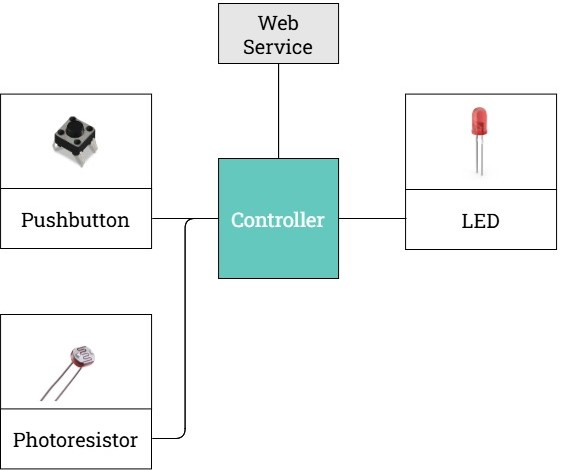
\includegraphics[width=\textwidth]{img/SystemDesign.jpg}
    \caption{System Design}
    \label{fig:SystemDesign}
\end{figure}

{Block Diagram của hệ thống được mô tả qua hình~\ref{fig:SystemDesign} cho biết thiết kế tổng quát của đồ án này. Theo đó, hệ thống gồm các thành phần sau: (1) Các thiết bị Input là Pushbutton (tên tiếng Việt: nút nhấn) để nhận tín hiệu bật tắt đèn của người dùng và Photoresistor (tên tiếng Việt: quang trở) để đo lường độ sáng của môi trường xung quanh hệ thống; (2) Thiết bị Output là đèn LED; (3) Controller đóng vai trò là thiết bị để nhận dữ liệu từ thiết bị Input, điều khiển thiết bị Output cũng như truyền và nhận không dây dữ liệu với Web Service; (4) Web Service là một ứng dụng web được triển khai nhằm mục đích cho người dùng biết được trạng thái hiện tại của đèn LED cũng như điều khiển đèn LED từ xa thông qua nút trên Website; (5) MQTT có vai trò là một giao thức trung gian giữa Controller và Website (cùng các thao tác, dịch vụ khác trên Internet nếu có); (6) LLMs (Generative AI) đóng vai trò là công cụ hỗ trợ để phân tích yêu cầu của người dùng thành lệnh điều khiển hệ thống và phản hồi người dùng. Các thành phần trên sẽ được mô tả chi tiết tại bảng~\ref{tab:components}.

\pagebreak
\subsection{Thiết kế chi tiết}\label{subsec:thiet_ke_chi_tiet}
\begin{table}[!h]
\centering
\small
\begin{tabular}{|p{0.6cm}|p{2.5cm}|p{3.5cm}|p{9cm}|}
\hline
\textbf{TT} & \textbf{Thành phần} & \textbf{Tên thiết bị/Công nghệ đề xuất} & \textbf{Cách thiết lập} \\ \hline
\textbf{1} & Controller & Kit Wifi BLE ESP32 NodeMCU-32S CH340 Ai-Thinker & 
- Nguồn và GND: Nối chân 5V và GND của ESP32 với nguồn điện và GND cho các thiết bị.

- Các Pin của ESP32: Nối với các thiết bị như LED và Pushbutton để truyền/nhận tín hiệu điều khiển và nối với cảm biến ánh sáng để đọc tín hiệu ánh sáng.\\ \hline
\textbf{2} & Web Service & Local Host, triển khai bằng Python (Panel) & 
- Triển khai trên Local Host và kết nối với Controller qua WiFi và trung gian là MQTT. 

- Gửi/Nhận Dữ liệu: Thiết lập kết nối giữa ESP32 và Web Service thông qua kết nối không dây WiFi với trung gian là giao thức MQTT để trao đổi dữ liệu điều khiển và giám sát trạng thái đèn LED từ Web Service đến ESP32 và ngược lại. \\ \hline
\textbf{3} & Pushbutton & 6x6x5 mm Miniature Micro Momentary Tactile Tact Touch Push Button & 
- Kết nối với ESP32: Nối một chân của Pushbutton với chân có thể đọc tín hiệu Digital của ESP32 và chân còn lại với GND.

- Điện trở: Thêm điện trở giữa chân Digital và GND để ổn định tín hiệu, tránh nhiễu. ESP32 sẽ đọc tín hiệu từ Pushbutton để điều khiển đèn LED.\\ \hline
\textbf{4} & Photoresistor & Lm393 Optical Photosensitive Ldr Light Sensor Module & 
- Kết nối với ESP32: Nối chân tín hiệu của module cảm biến ánh sáng (LDR) với chân có thể đọc tín hiệu Analog In của ESP32. Nối chân VCC và GND của module với chân 5V và GND của ESP32.

- Đọc cường độ ánh sáng: ESP32 sẽ đọc giá trị từ LDR để xác định trạng thái sáng tối của môi trường xung quanh. \\ \hline
\textbf{5} & LED & 5mm Color Led & 
- Kết nối với ESP32: Nối chân dương của LED với chân có thể ghi tín hiệu Digital của ESP32 qua một điện trở để bảo vệ LED. Nối chân âm của LED với GND.

- Điều khiển Bật/Tắt: ESP32 sẽ điều khiển LED dựa trên tín hiệu từ cảm biến ánh sáng hoặc Pushbutton hoặc lệnh bật tắt từ Website. \\ \hline

\textbf{6} & MQTT & HiveMQ & 
- Có nhiệm vụ là trung gian nhận tín hiệu từ hệ thống IoT để các dịch vụ khác có thể theo dõi được dữ liệu các thiết bị và gửi tín hiệu điều khiển của người dùng đến hệ thống IoT. 

- Cần đăng ký tài khoản và topic để tăng tính bảo mật cho dữ liệu.\\ \hline

\textbf{7} & LLMs (Generative AI) & Các mô hình ngôn ngữ lớn & 
- Có nhiệm vụ tiếp nhận yêu cầu của người dùng (dưới dạng văn bản), phân tích thành lệnh điều khiển thiết bị IoT và tạo văn bản hồi đáp/trả lời người dùng. 

- Cần đăng ký tài khoản và tạo API key để sử dụng. Cũng lưu ý rằng đối với tài khoản miễn phí thì API key có số quota khá hạn chế nếu có nhu cầu dùng nhiều.\\ \hline
\end{tabular}

\caption{Danh sách các thành phần của hệ thống}
\label{tab:components}

\end{table}

Bảng~\ref{tab:components} cho biết mô tả chi tiết về các thành phần Controller, Web Service, Pushbutton, Photoresistor, đèn LED, MQTT, LLMs (Generative AI) của hệ thống đã được thiết kế trên System Design ở hình~\ref{fig:SystemDesign}. Theo đó, bảng~\ref{tab:components} đưa ra đề xuất thiết bị, công nghệ phù hợp cũng như cách thiết lập các thiết bị đó để có cơ sở thiết kế chi tiết và triển khai ở các giai đoạn sau (như thiết kế sơ đồ mạch điện, FSM, sơ đồ truyền nhận dữ liệu, triển khai giả lập và triển khai trên thiết bị thật). 

\subsection{Sơ đồ mạch điện đề xuất}
\begin{figure}[H]
    \centering
    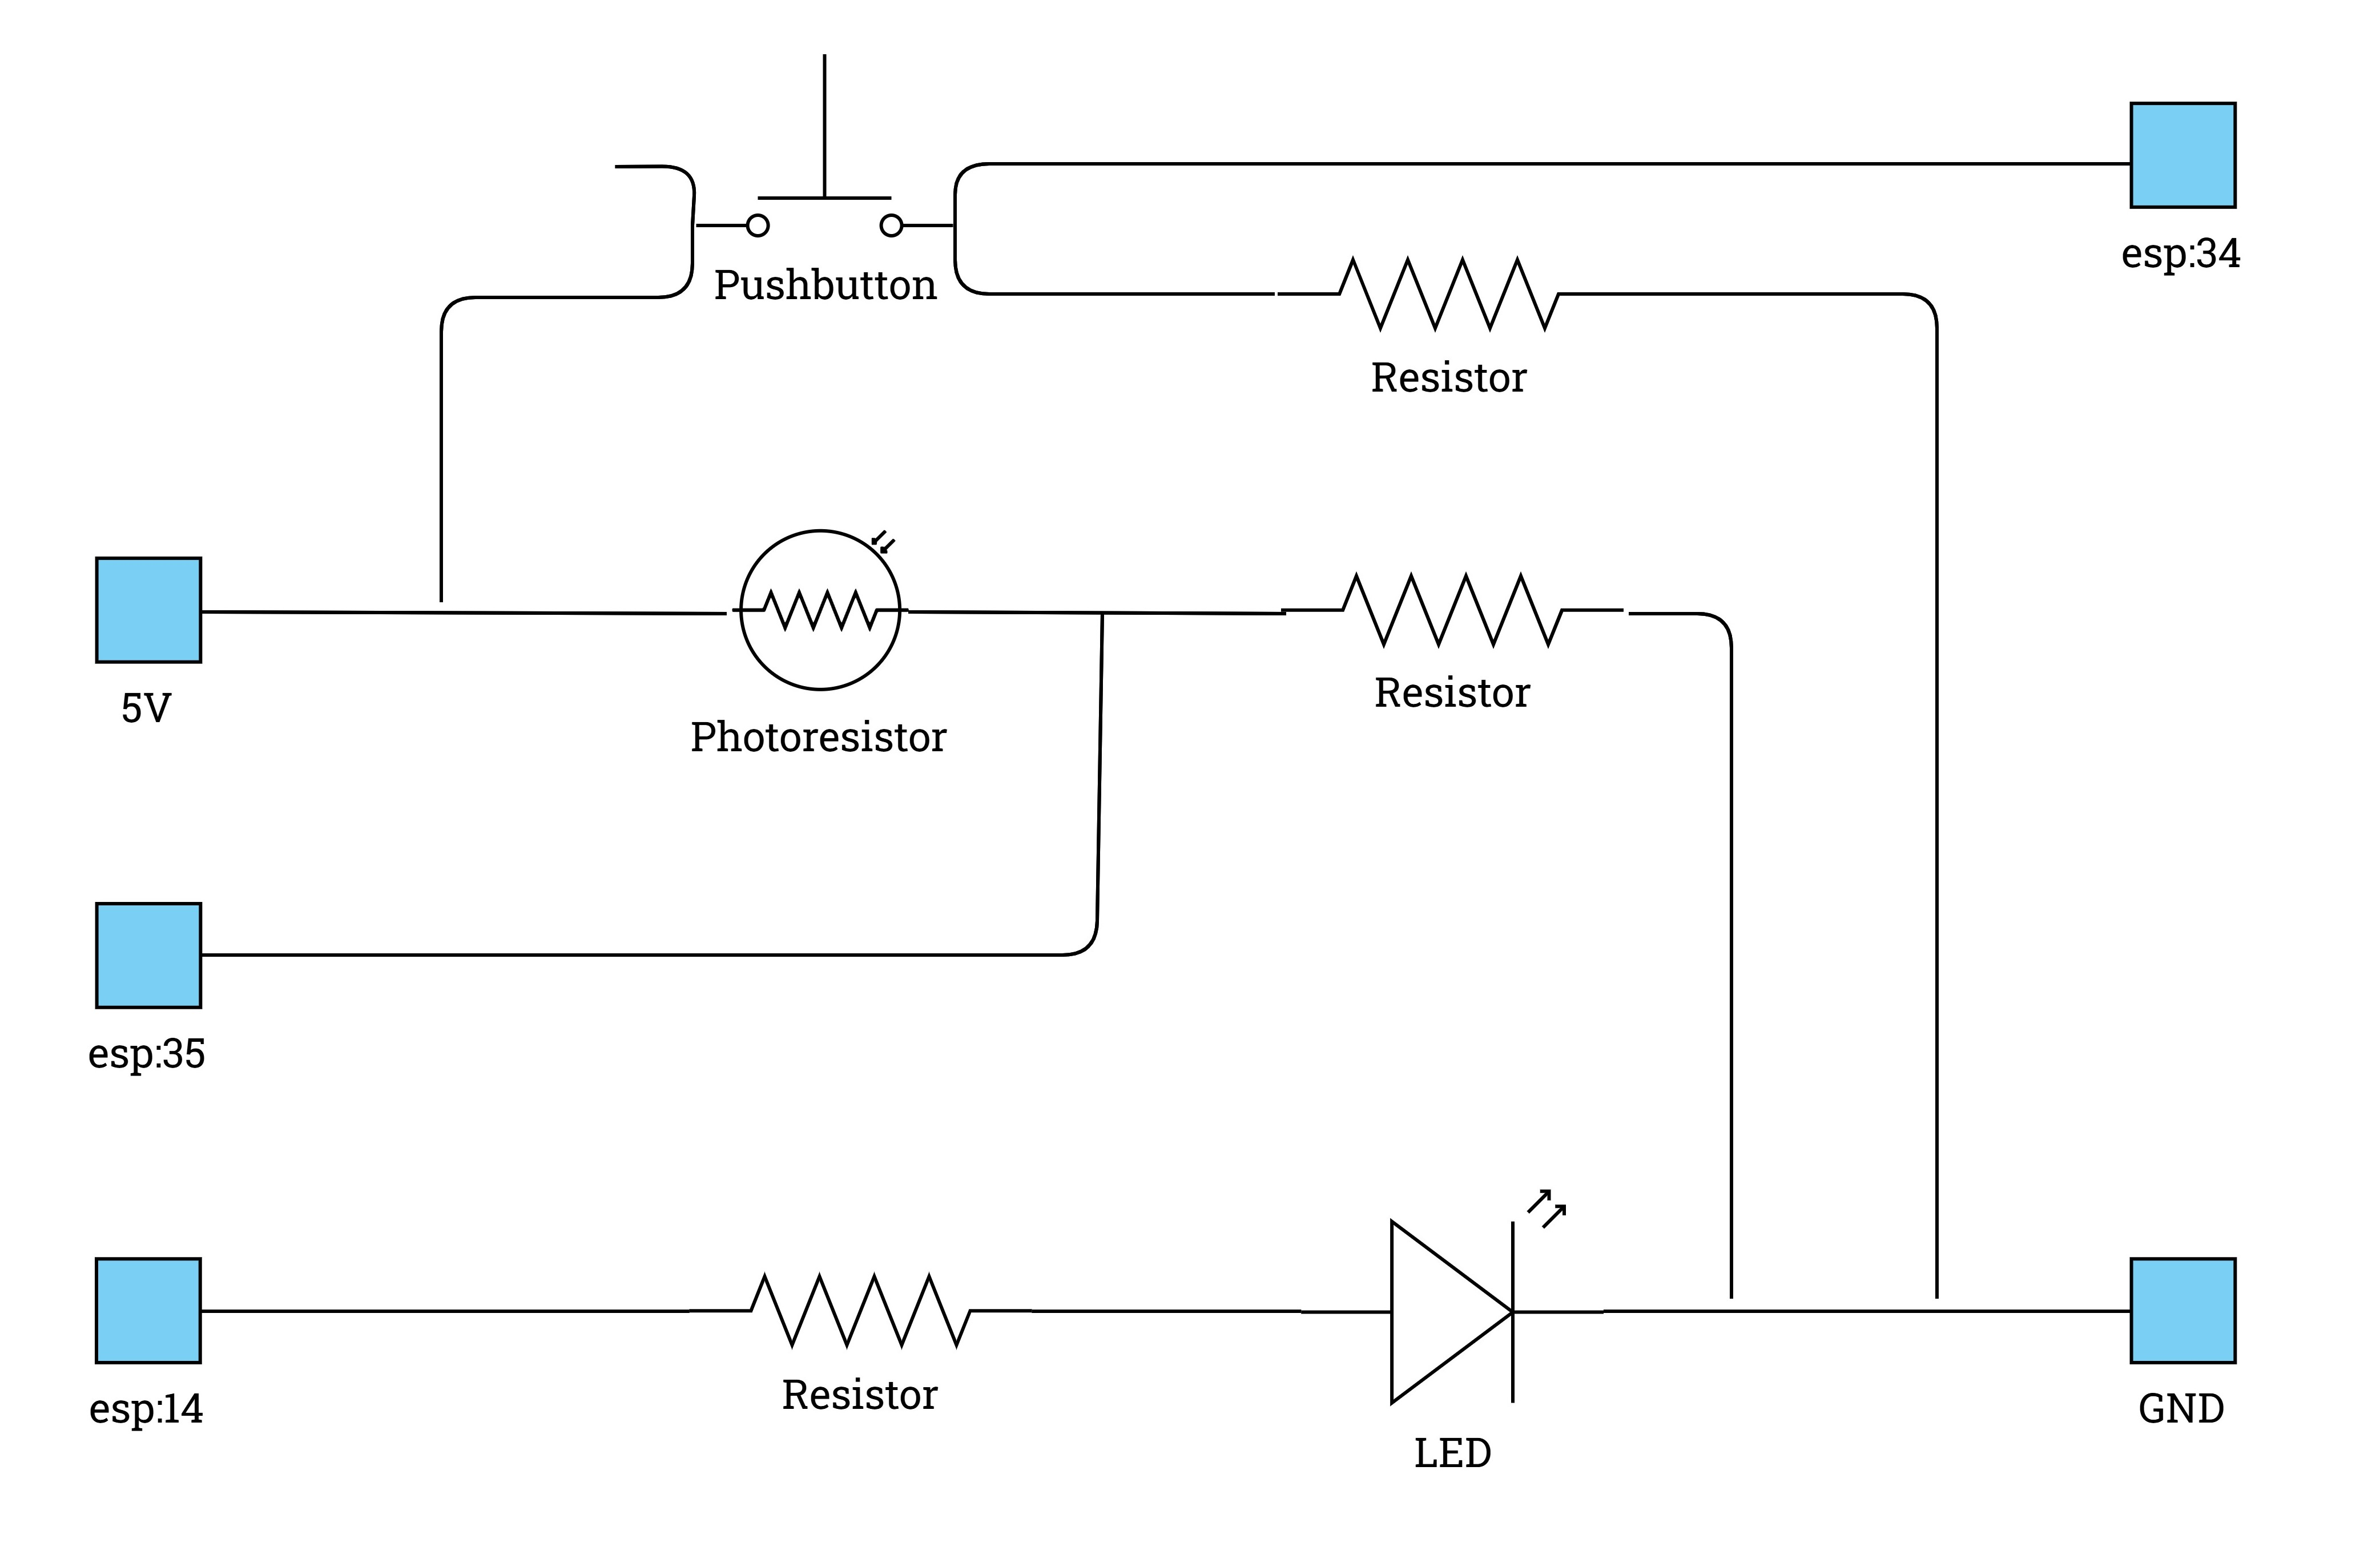
\includegraphics[width=\textwidth]{img/Circuit.jpg}
    \caption{Sơ đồ mạch điện dự kiến triển khai hệ thống}
    \label{fig:Circuit}
\end{figure}

Sơ đồ mạch điện trên hình~\ref{fig:Circuit} mô tả một mạch bao gồm một nút nhấn (Pushbutton), một quang trở (Photoresistor) và một đèn LED được kết nối với các chân của vi điều khiển Kit Wifi BLE ESP32 NodeMCU-32S CH340 Ai-Thinker (sau đây gọi tắt là ESP32). Các chân ESP32 được sử dụng bao gồm: chân nguồn 5V và GND; các chân esp:14, esp:34, esp:35. Nguồn điện 5V được cung cấp cho mạch qua chân 5V và chân GND. Khi nút nhấn được bấm, mạch cho phép dòng điện đi qua các điện trở và quang trở đến chân esp:35 để đo ánh sáng từ quang trở. Chân esp:34 được sử dụng để theo dõi trạng thái của nút nhấn và chân esp:14 được sử dụng để điều khiển đèn LED. Đèn LED, quang trở và nút nhấn được mắc nối tiếp qua các điện trở để hạn chế dòng điện nhằm bảo vệ các thiết bị trên khỏi dòng điện quá lớn và đảm bảo mạch hoạt động ổn định.


\subsection{Sơ đồ máy trạng thái hữu hạn (FSM - Finite-state Machine)}
\begin{figure}[H]
    \centering
    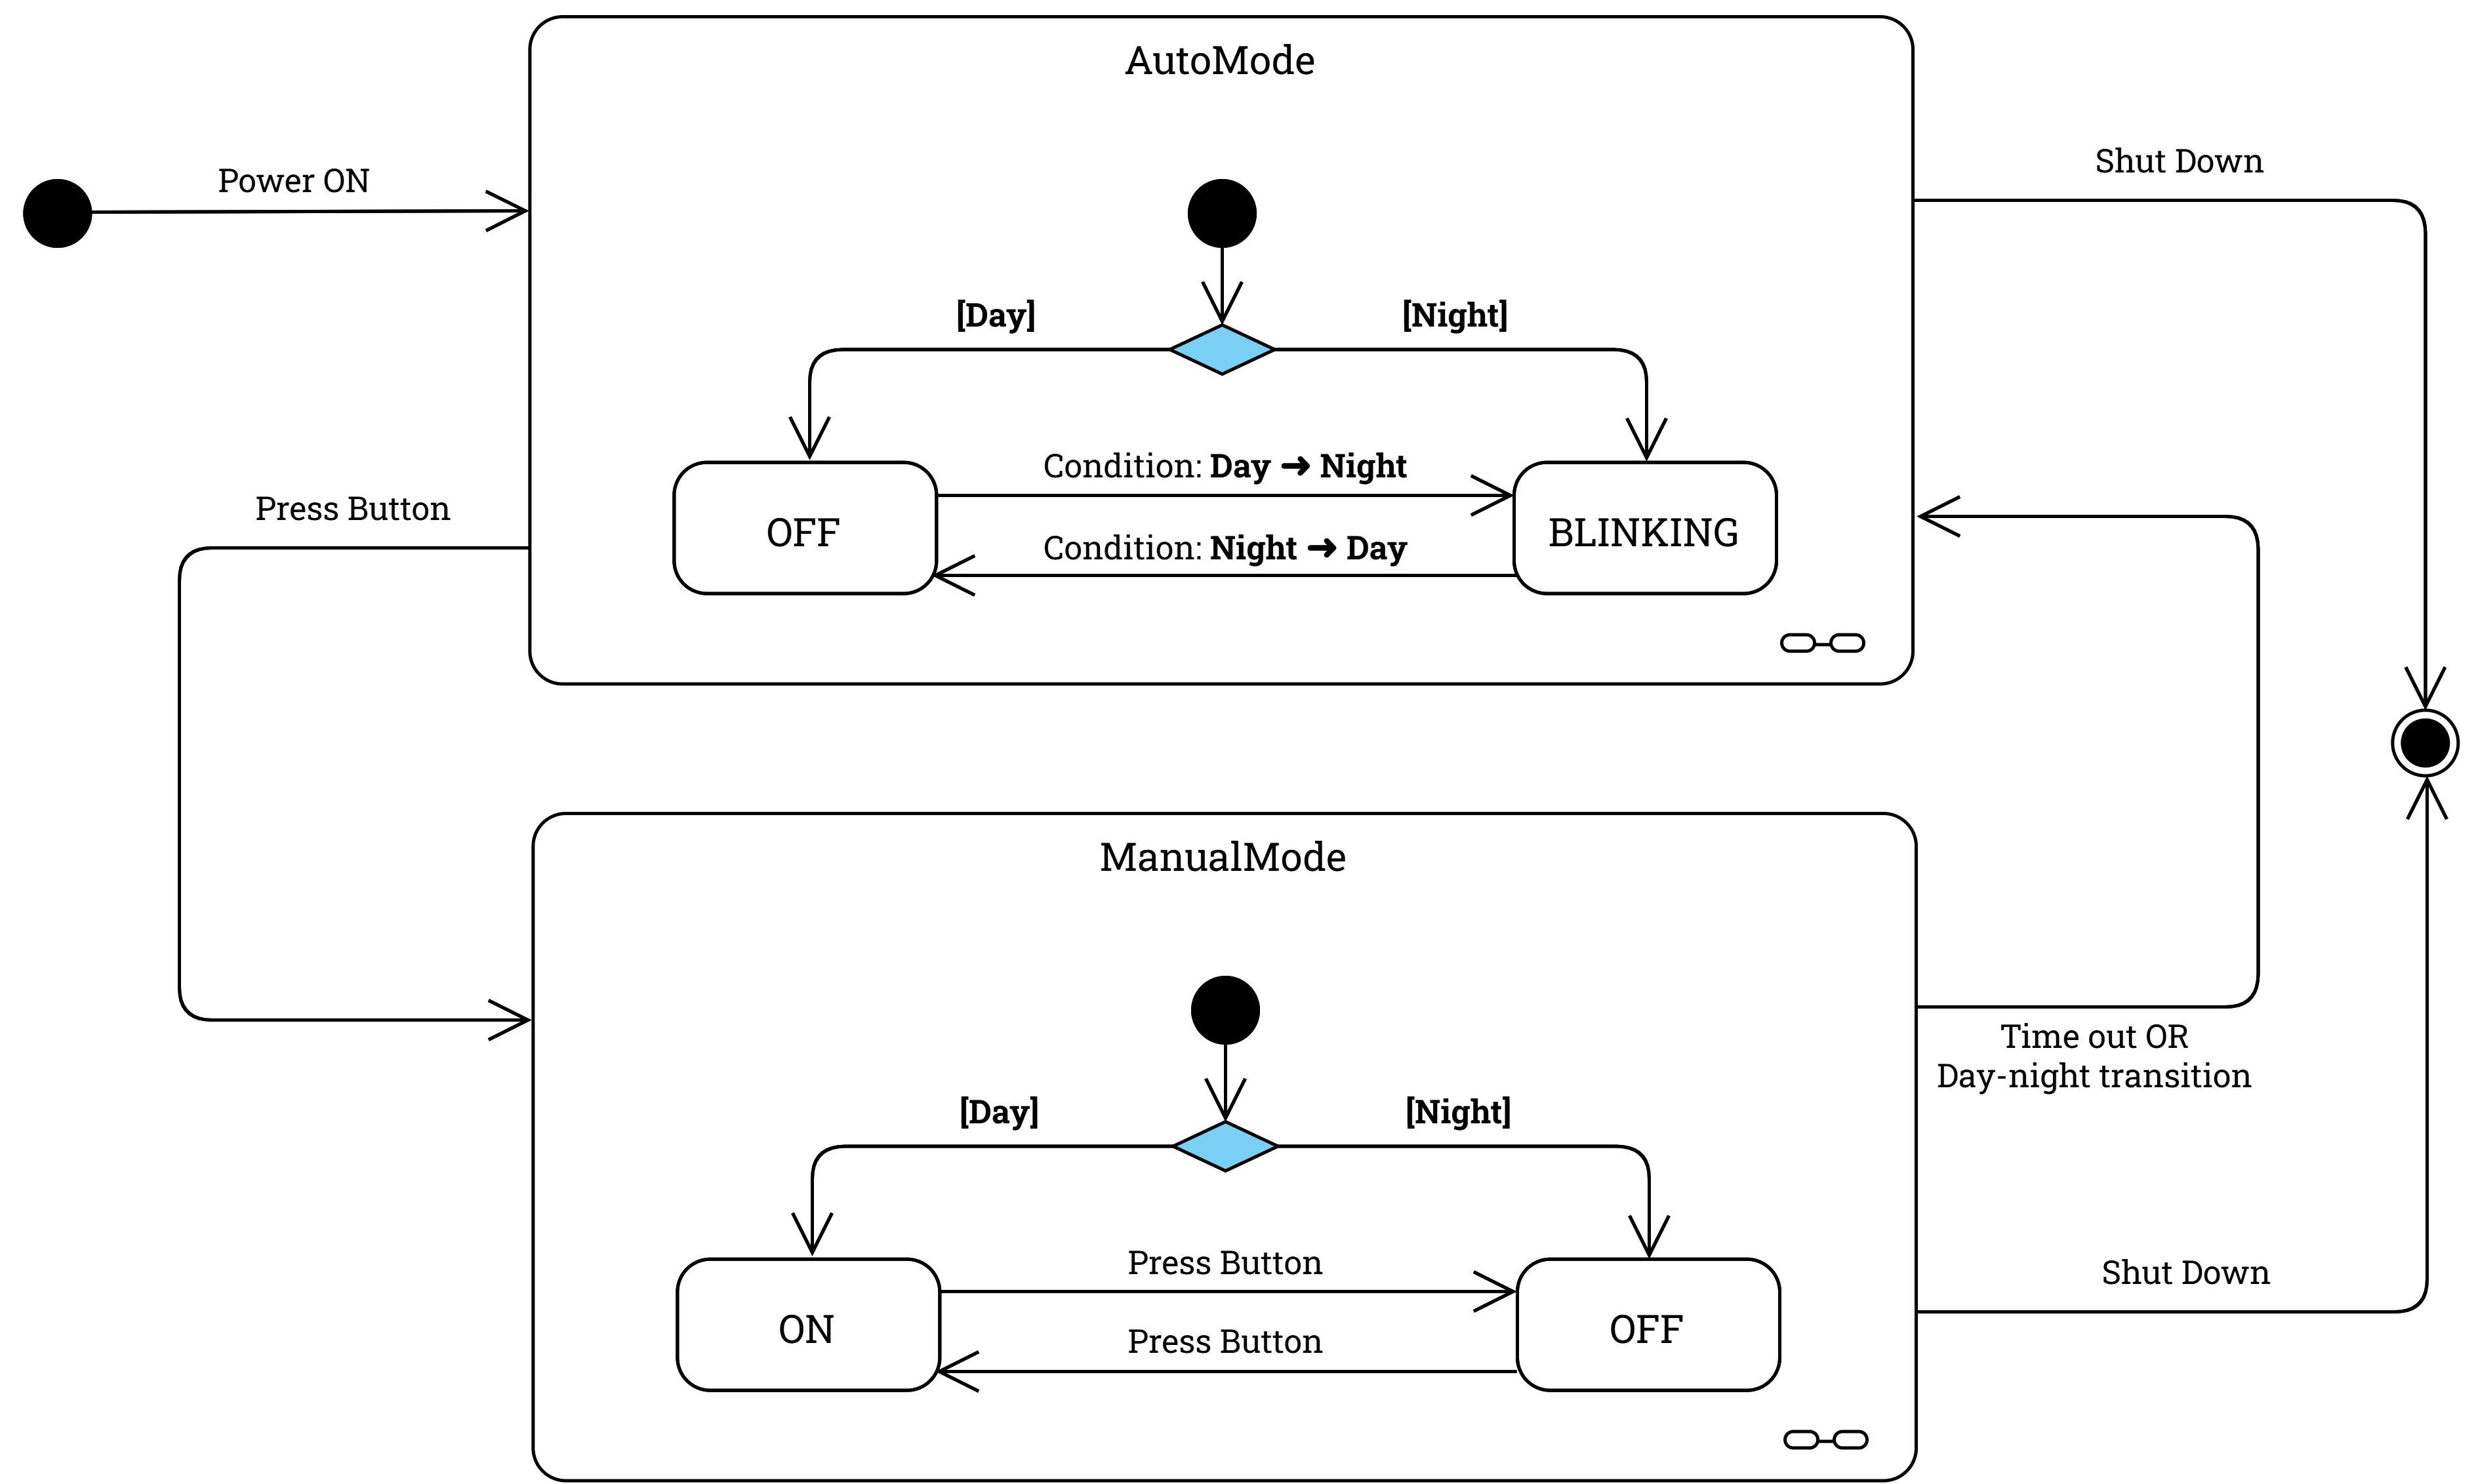
\includegraphics[scale=0.16]{img/FSM-2.jpg}
    \caption{Sơ đồ máy trạng thái hữu hạn của đèn LED trong hệ thống}
    \label{fig:FSM}
\end{figure}

Sơ đồ FSM (Finite State Machine) ở hình~\ref{fig:FSM}  mô tả hệ thống điều khiển đèn với hai chế độ: AutoMode và ManualMode. Khi ESP32 được nạp điện (Power ON), chế độ AutoMode được kích hoạt. Trong AutoMode, nếu là ban ngày (Day), đèn sẽ ở trạng thái OFF; nếu chuyển sang ban đêm (Night), đèn sẽ chuyển sang trạng thái BLINKING. Khi trời sáng trở lại (Night sang Day), đèn sẽ quay về trạng thái OFF và ngược lại, khi trời chuyển từ sáng sang tối (Day sang Night) thì đèn sẽ sang trạng thái BLINKING. Khi người dùng nhấn nút, hệ thống chuyển sang ManualMode.\\

Trong ManualMode, đèn có thể được bật (ON) hoặc tắt (OFF) thông qua nút nhấn. Ở trạng thái ON, nếu nhấn nút lần nữa, đèn sẽ chuyển sang OFF và ngược lại. Hệ thống sẽ quay lại AutoMode khi có sự chuyển đổi từ ngày sang đêm, đêm sang ngày hoặc khi hết thời gian quy định (timeout). Ở bất kỳ trạng thái nào, hệ thống sẽ kết thúc hoạt động khi bị ngắt nguồn (tức là Shut Down).\\

Sự chuyển đổi trạng thái của sơ đồ FSM ở hình~\ref{fig:FSM} được mô tả thông qua bảng~\ref{tab:FSM}: Bảng chuyển đổi trạng thái của đèn LED trong hệ thống. 

\begin{table}[H]
\centering
\small
\begin{tabular}{|p{2.3cm}|p{3cm}|p{4cm}|p{2cm}|p{4cm}|}
\hline

\textbf{Current State} & \textbf{Input} & \textbf{Condition} & \textbf{Next State} & \textbf{Output} \\ \hline
{Initial State}                                & {Power ON}                            & {Current Condition == Day}                & {AutoMode - OFF}                           & Start AutoMode                            \\ \hline
{Initial State}                                & {Power ON}                            & {Current Condition == Night}              & {AutoMode - BLINKING}                      & Start blinking LED with AutoMode          \\ \hline
{AutoMode - OFF}                               & {Day → Night Transition}              & {-}                                       & {AutoMode - BLINKING}                      & Start blinking LED                        \\ \hline
{AutoMode - BLINKING}                          & {Night → Day Transition}              & {-}                                       & {AutoMode -  OFF}                          & Turn off LED                              \\ \hline
{AutoMode - OFF}                               & {Press Button}                        & {-}                                       & {ManualMode - ON}                          & Switch to ManualMode and turn on LED      \\ \hline
AutoMode - BLINKING                                                 & Press Button                                               & -                                                              & ManualMode - OFF                                                & Switch to ManualMode and turn off LED     \\ \hline
ManualMode - ON                                                     & Press Button                                               & \textit{-}                                                     & ManualMode - OFF                                                & Turn off LED                              \\ \hline
ManualMode - OFF                                                    & Press Button                                               & -                                                              & ManualMode - ON                                                 & Turn on LED                               \\ \hline
ManualMode - ON                                                     & Day-Night Transition                                       & Current Condition == Day                                       & AutoMode - OFF                                                  & Switch to AutoMode and turn off LED       \\ \hline
ManualMode - ON                                                     & Day-Night Transition                                       & Current Condition == Night                                     & AutoMode - BLINKING                                             & Switch to AutoMode and start blinking LED \\ \hline
ManualMode - ON                                                     & Timeout                                                    & Current Condition == Day                                       & AutoMode - OFF                                                  & Switch to AutoMode and turn off LED       \\ \hline
ManualMode - ON                                                     & Timeout                                                    & Current Condition == Night                                     & AutoMode - BLINKING                                             & Switch to AutoMode and start blinking LED \\ \hline
ManualMode - OFF                                                    & Day-Night Transition                                       & Current Condition == Day                                       & AutoMode - OFF                                                  & Switch to AutoMode and turn off LED       \\ \hline
ManualMode - OFF                                                    & Day-Night Transition                                       & Current Condition == Night                                     & AutoMode - BLINKING                                             & Switch to AutoMode and start blinking LED \\ \hline
ManualMode - OFF                                                    & Timeout                                                    & Current Condition == Day                                       & AutoMode - OFF                                                  & Switch to AutoMode and turn off LED       \\ \hline
ManualMode - OFF                                                    & Timeout                                                    & Current Condition == Night                                     & AutoMode - BLINKING                                             & Switch to AutoMode and start blinking LED \\ \hline
AutoMode - OFF                                                      & Shut Down                                                  & -                                                              & Shutdown State                                                               & Shut Down System                          \\ \hline
AutoMode - BLINKING                                                 & Shut Down                                                  & -                                                              & Shutdown State                                                               & Shut Down System and turn off LED         \\ \hline
ManualMode - ON                                                     & Shut Down                                                  & -                                                              & Shutdown State                                                               & Shut Down System and turn off LED         \\ \hline
ManualMode - OFF                                                    & Shut Down                                                  & -                                                              & Shutdown State                                                               & Shut Down System                          \\ \hline
\end{tabular}
\caption{Bảng chuyển đổi trạng thái của đèn LED trong hệ thống}
\label{tab:FSM}
\end{table}

Căn cứ FSM trên hình~\ref{fig:FSM}, bảng~\ref{tab:FSM} ở trên mô tả chuyển đổi trạng thái của đèn LED trong hệ thống. 


\subsection{Sơ đồ truyền nhận dữ liệu}
\begin{figure}[H]
    \centering
    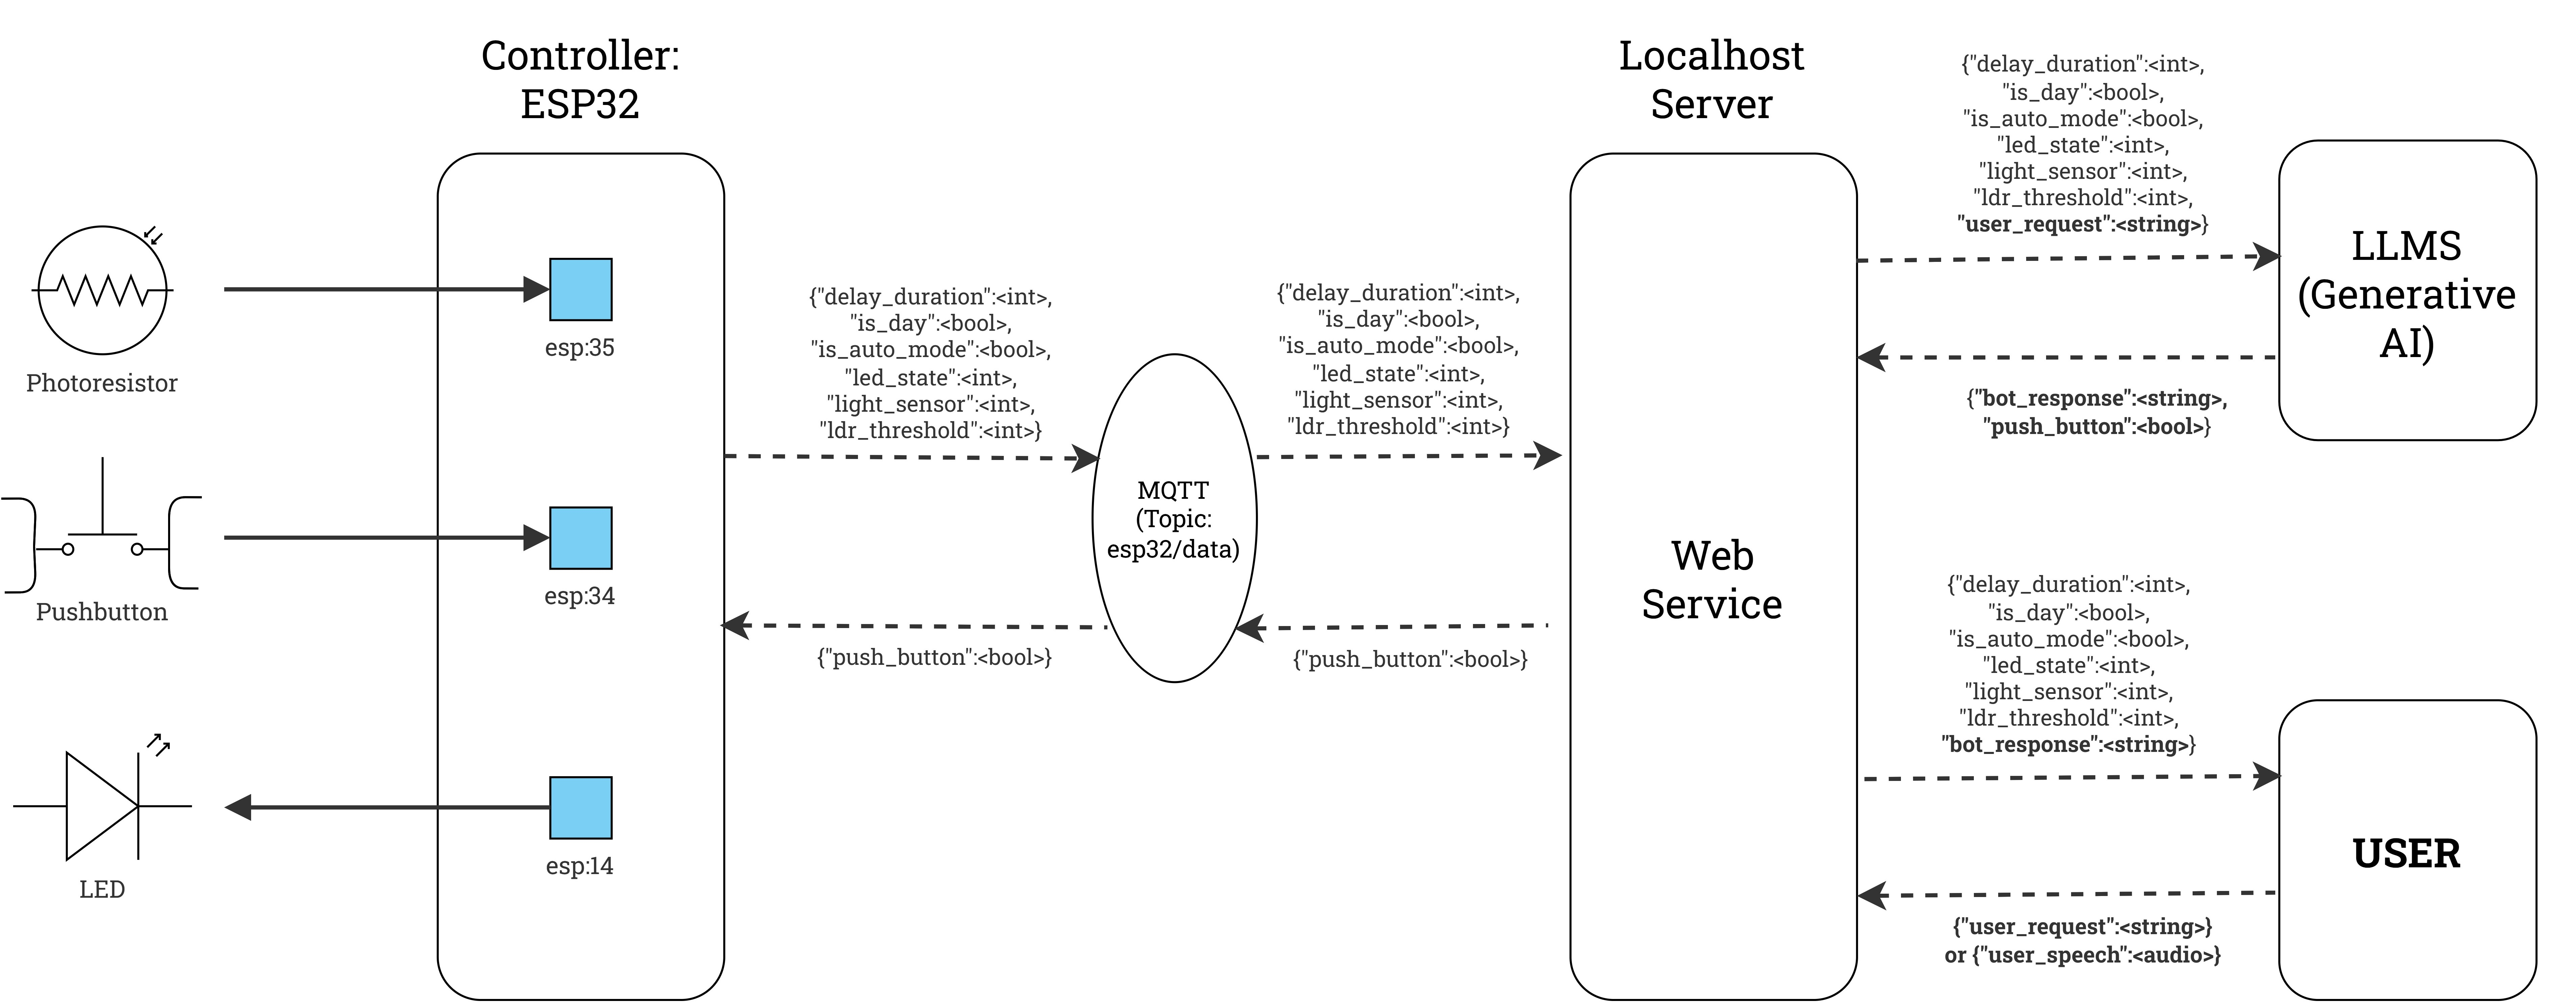
\includegraphics[width=\textwidth]{img/Data.jpg}
    \caption{Sơ đồ truyền nhận dữ liệu giữa các thiết bị, Controller và Web Server}
    \label{fig:Data}
\end{figure}

Sơ đồ tại hình~\ref{fig:Data} mô tả quá trình truyền nhận dữ liệu giữa ESP32 và Web Service qua giao thức MQTT bằng truyền dữ liệu không dây WiFi. ESP32 đọc giá trị từ quang trở (qua cổng esp:35), nút nhấn (qua cổng esp:34) và căn cứ vào các dữ liệu đó để điều khiển đèn LED (qua cổng esp:14). Trong quá trình xử lý, ESP32 gửi liên tục các thông tin hiện thời về thời gian timeout (đơn vị: second), chế độ đang vận hành hệ thống (AutoMode hay ManualMode), điều kiện ánh sáng môi trường (chỉ số quang trở tương ứng Day hay Night) và trạng thái đèn (đang tắt - OFF hay đang sáng - ON hay đèn có đang Blinking không) đến Web Service thông qua giao thức MQTT (Topic: esp32/data) qua truyền không dây WiFi dưới dạng 1 JSON. Ở chiều ngược lại, Web Service cũng có thể gửi lệnh điều khiển dưới hình thức người dùng thao tác trên Website (nhập text hoặc voice) và Web Service sẽ gọi LLMs (Generative AI) để xử lý thành lệnh và phản hồi người dùng và gửi tới ESP32 (vẫn thông qua topic esp32/data của MQTT) để điều khiển hệ thống. Việc truyền nhận dữ liệu giữa ESP32 và Web Service thông qua MQTT và WiFi được diễn ra liên tục nhằm cập nhật chính xác nhất trạng thái hiện thời của hệ thống. \\

Sơ đồ tại hình~\ref{fig:Data} được mô tả chi tiết và rõ ràng hơn thông qua các phần~\ref{subsec:data_in_UNO},~\ref{subsec:data_UNO_to_Web},~\ref{subsec:data_Web_to_UNO}.

\subsubsection{Truyền dữ liệu, tín hiệu giữa Controller và các thiết bị}\label{subsec:data_in_UNO}
%\textbf{Các thiết bị truyền dữ liệu, tín hiệu đến Controller:} 
\begin{table}[H]
\centering
\small
\begin{tabular}{|p{2.5cm}|p{2.5cm}|p{2.5cm}|p{2.5cm}|p{4.5cm}|}
\hline
{\textbf{Thiết bị}}            & {\textbf{Pin giao tiếp}} & {\textbf{Điện thế}} & {\textbf{Giá trị}} & {\textbf{Ý nghĩa}}                                 \\ \hline
{Photoresistor}                & {esp:35}                     & {0V đến 5V}         & {0 đến 1023}       & {Cường độ ánh sáng của môi trường xung quanh hệ thống} \\ \hline
{}                             & {}                       & {0V}                & {LOW}              & {Released}                                         \\ \cline{3-5} 
\multirow{-2}{*}{{Pushbutton}} & \multirow{-2}{*}{{esp:34}}   & {5V}                & {HIGH}             & {Pressed}                                          \\ \hline

\end{tabular}
\caption{Các thiết bị truyền dữ liệu, tín hiệu đến Controller}
\label{tab:data_photo_push}
\end{table}


%\textbf{Các thiết bị nhận tín hiệu từ Controller: }
\begin{table}[H]
\centering
\small
\begin{tabular}{|p{2.5cm}|p{2.5cm}|p{2.5cm}|p{2.5cm}|p{4.5cm}|}
\hline
{\textbf{Thiết bị}}     & {\textbf{Pin giao tiếp}} & {\textbf{Điện thế}} & {\textbf{Giá trị}} & {\textbf{Ý nghĩa}}         \\ \hline
{}                      & {}                       & {5V}                & {HIGH}             & {ON: tức bật sáng đèn LED} \\ \cline{3-5} 
\multirow{-2}{*}{{LED}} & \multirow{-2}{*}{{esp:14}}   & {0V}                & {LOW}              & {OFF: tức tắt đèn LED}     \\ \hline
\end{tabular}
\caption{Các thiết bị nhận tín hiệu từ Controller}
\label{tab:data_LED}
\end{table}

Người đọc có thể tham khảo sơ đồ mạch điện trên hình~\ref{fig:Circuit}, sơ đồ truyện nhận dữ liệu trên hình~\ref{fig:Data} và mạch giả lập hệ thống trên Wokwi tại hình~\ref{fig:tinkercad} để có góc nhìn rộng hơn về các thiết bị này và các pin liên quan được đề cập trong bảng~\ref{tab:data_photo_push} và bảng~\ref{tab:data_LED}. 

\pagebreak
\subsubsection{Truyền dữ liệu, tín hiệu từ Controller đến Web Service}\label{subsec:data_UNO_to_Web}
\textbf{Cấu trúc JSON:}
    \begin{lstlisting}
{"delay_duration":<int>,"is_day":<bool>,"is_auto_mode":<bool>,"led_state":<int>,"light_sensor":<int>,"ldr_threshold":<int>}\end{lstlisting}

Trường JSON được gửi liên tục đến Topic esp32/data của HiveMQ MQTT bao gồm các thông tin cần thiết để hệ thống điều khiển và giám sát trạng thái hoạt động của đèn LED thông minh:
\begin{itemize}
    \item \textbf{\texttt{delay\_duration}}: Thời gian chờ trước khi thực hiện thay đổi trạng thái đèn hoặc chuyển chế độ từ Manual Mode sang Auto Mode nếu không có thao tác từ người dùng. Giá trị này được gửi bằng đơn vị giây (giá trị nguyên).
    \item \textbf{\texttt{is\_day}}: Xác định điều kiện ánh sáng môi trường xung quanh (sáng hoặc tối). Giá trị true biểu thị ban ngày, và false biểu thị ban đêm.
    \item \textbf{\texttt{is\_auto\_mode}}: Chế độ hiện tại của hệ thống. Giá trị true biểu thị chế độ tự động (Auto Mode), và false biểu thị chế độ thủ công (Manual Mode).
    \item \textbf{\texttt{led\_state}}: Trạng thái hiện tại của đèn LED. Giá trị 0 biểu thị đèn tắt (Off), 1 biểu thị đèn sáng (On), và 2 biểu thị đèn nhấp nháy (Blinking).
    \item \textbf{\texttt{light\_sensor}}: Giá trị ánh sáng đọc được từ cảm biến, giúp hệ thống phân biệt giữa ngày và đêm.
    \item \textbf{\texttt{ldr\_threshold}}: Giá trị ngưỡng ánh sáng cài đặt để xác định ngày hay đêm. Nếu giá trị ánh sáng từ cảm biến lớn hơn hoặc bằng ngưỡng này, hệ thống xác định là ban đêm; ngược lại là ban ngày.
\end{itemize}



\pagebreak
\subsubsection{Truyền dữ liệu, tín hiệu từ Web Service đến Controller}\label{subsec:data_Web_to_UNO}

\textbf{Cấu trúc JSON:}
    \begin{lstlisting}
{"push_button":<bool>}\end{lstlisting}

Trường JSON này được gửi liên tục đến Topic esp32/data của HiveMQ MQTT. Theo đó dữ liệu này được phân tích dựa trên user\_request (dạng text hoặc text sau khi Speech to Text voice của người dùng) mà LLMs phân tích. LLMs sẽ gửi xem là yêu cầu của người dùng cần nhấn nút hay không, cũng như tạo response để phản hồi cho người dùng. 

\pagebreak
\section{Đề xuất các giải pháp}
{% \begin{table}[H]
\centering
\small
\begin{longtable}{|p{2.3cm}|p{3.2cm}|p{3.2cm}|p{3.2cm}|p{3.5cm}|}
\hline
\textbf{Component /Module} & \textbf{Giải pháp 1} & \textbf{Giải pháp 2} & \textbf{Giải pháp 3} & \textbf{Quyết định giải pháp} \\ \hline
\endfirsthead

\hline
\textbf{Component /Module} & \textbf{Giải pháp 1} & \textbf{Giải pháp 2} & \textbf{Giải pháp 3} & \textbf{Quyết định giải pháp} \\ \hline
\endhead

\hline
Controller 
& \textbf{Arduino Uno R3 ATmega328}


- Chi phí: $\sim$100.000 VNĐ


- Dễ lập trình và mở rộng


- Phù hợp cho các hệ thống cơ bản & \textbf{Raspberry Pi 3B+}


- Chi phí: \textgreater{}1.890.000 VNĐ


- Có khả năng xử lý cao hơn


- Hỗ trợ hệ điều hành


- Phù hợp cho các ứng dụng phức tạp & \textbf{Kit Wifi BLE ESP32 NodeMCU-32S CH340 Ai-Thinker}


- Chi phí: $\sim$190.000 VNĐ


- Tích hợp sẵn Wifi và Bluetooth


- Phù hợp cho IoT và hệ thống có kết nối mạng

& \textbf{Kit Wifi BLE ESP32 NodeMCU-32S CH340 Ai-Thinker}


Đáp ứng đủ yêu cầu, chi phí hợp lý, dễ sử dụng. \\ \hline

Web Service 

& \textbf{Local Host (Panel Python)}


- Triển khai cục bộ trên máy tính


- Chi phí: Miễn phí


- Thích hợp cho giai đoạn thử nghiệm & \textbf{Cloud Hosting}


- Dùng nền tảng đám mây (AWS, Azure)


- Chi phí: phí duy trì hàng tháng


- Khả năng mở rộng tốt


- Truy cập từ xa tiện lợi & \textbf{Raspberry Pi làm Server}


- Kết nối trực tiếp với cảm biến


- Chi phí thiết lập cao hơn


- Phù hợp cho các hệ thống nhỏ gọn, tự chủ & \textbf{Local Host (Panel Python)}


Chi phí thấp và đáp ứng được yêu cầu cơ bản của đồ án. \\ \hline

Pushbutton 

& \textbf{6x6x5 mm Tactile Push Button}


- Chi phí thấp


- Đơn giản, dễ lắp đặt & \textbf{Công tắc cảm ứng chạm}


- Chi phí cao hơn (khoảng 20.000 VNĐ)


- Tạo trải nghiệm hiện đại


- Có thể nhúng vào thiết kế đẹp mắt & \textbf{Công tắc nhấn IP67}


- Chống nước và bụi, phù hợp môi trường ngoài trời


- Chi phí cao hơn (khoảng 20.000 VNĐ)


- Độ bền cao 

& \textbf{6x6x5 mm Tactile Push Button}


Đơn giản, chi phí thấp, dễ sử dụng. \\ \hline

Photoresistor 

& \textbf{Lm393 Optical Photosensitive LDR}


- Chi phí thấp (khoảng 20.000 VNĐ)


- Độ nhạy cao với ánh sáng


- Dễ kết nối với Arduino & \textbf{Cảm biến ánh sáng BH1750}


- Chi phí cao hơn ($\sim$40.000 VNĐ)


- Độ chính xác cao hơn


- Kết nối qua giao thức I2C 

& \textbf{Cảm biến TSL2561}


- Chi phí khoảng  140.000 VNĐ


- Đo ánh sáng với độ chính xác cao, dải rộng


- Phù hợp cho các dự án cần đo ánh sáng chính xác 

& \textbf{Lm393 Optical Photosensitive LDR}


Đáp ứng yêu cầu chi phí thấp và dễ sử dụng trong môi trường ánh sáng đơn giản. \\ \hline

LED 

& \textbf{5mm Color LED}


- Đơn giản, dễ lắp đặt


- Chi phí thấp ($\sim$9.000 VNĐ/30 đèn) 

& \textbf{LED RGB}


- Đổi màu, tạo hiệu ứng


- Chi phí cao hơn ($\sim$16.000 VNĐ)


- Phù hợp nếu cần thay đổi màu sắc 

& \textbf{Grove - LED Button}


- Có tích hợp sẵn kèm theo với Pushbutton.


- Tuổi thọ sử dụng cao hơn (100.000 lần bật tắt)


- Chi phí cao hơn ($\sim$66.000 VNĐ) 

& \textbf{5mm Color LED}


Chi phí thấp, đáp ứng yêu cầu chiếu sáng cơ bản. \\ \hline

\caption{Danh sách đề xuất các giải pháp cho hệ thống}
\label{tab:sugg}
\end{longtable}

% \end{table}
}

Bảng~\ref{tab:sugg} đưa ra mô tả các giải pháp khả thi cho các Component/Module của hệ thống. Việc đa dạng hóa các giải pháp giúp hệ thống có nhiều phương án dự phòng, nhiều phương án phát triển hệ thống theo các hướng đi mới hiệu quả hơn và có khả năng khắc phục được những hạn chế còn tồn đọng (nếu có). Cần căn cứ vào Đặc tả yêu cầu và những ràng buộc, hạn chế cũng như bản thiết kế hệ thống để có thể đưa ra được \textit{Quyết định giải pháp} hợp lý nhất cho quá trình phát triển hệ thống ở thời điểm hiện tại. Các giải pháp có chi phí thấp, dễ mua, dễ thiết lập và sử dụng, có phiên bản giả lập, đáp ứng đầy đủ ở mức cơ bản mà đặc tả yêu cầu đề ra là những giải pháp được chọn hiện tại dựa trên cơ sở như còn gặp nhiều hạn chế về kinh phí và trình độ hiện tại của lập trình viên hệ thống. 


\pagebreak
\section{Kế hoạch kiểm thử}
\subsection{Kiểm tra từng thành phần}
\begin{table}[h!]
\centering
\small
\begin{tabular}{|p{4cm}|p{10cm}|}
\hline
\textbf{Thành phần} & \textbf{Kiểm tra} \\ \hline
Controller (Kit Wifi BLE ESP32 NodeMCU-32S CH340 Ai-Thinker) & - Kiểm tra Controller khởi tạo đúng và tất cả các chân (pins) được cấu hình theo thiết kế. \\
& - Kiểm tra giao tiếp nối tiếp dữ liệu thông qua kết nối không dây WiFi để đảm bảo khả năng truyền dữ liệu chính xác. \\ \hline
Web Service (Local Host với Panel của Python) & - Kiểm tra các thành phần của chương trình xử lý yêu cầu và trả về kết quả như mong đợi.


- Giả lập dữ liệu gửi từ ESP32 và kiểm tra dữ liệu được nhận và hiển thị chính xác. Đồng thời xuất kết quả gửi từ chương trình trên terminal và MQTT để đảm bảo tính chính xác của dữ liệu gửi đến ESP32. \\ \hline
Pushbutton (6x6x5 mm Miniature Micro Momentary Tactile Tact Push Button) & - Xác nhận nút nhấn ghi nhận trạng thái thay đổi (nhấn và thả) và gửi dữ liệu đến Controller. \\ \hline
Photoresistor (Lm393 Optical Photosensitive LDR Light Sensor Module) & - Đo độ nhạy sáng và đảm bảo đọc giá trị analog chính xác. 


- Kiểm tra khả năng của quang trở để phân biệt giữa ngưỡng sáng ngày và đêm. (Đặc biệt tại môi trường dự kiến triển khai hệ thống) \\ \hline
LED (5mm Color LED) & - Kiểm tra đèn LED phản hồi tín hiệu kỹ thuật số cho các trạng thái BẬT, TẮT và NHẤP NHÁY. \\
& - Kiểm tra độ sáng/độ rõ của đèn LED trong điều kiện bình thường. \\ \hline
\end{tabular}
\caption{Kiểm tra các thành phần hệ thống}
\label{tab:component_checks}
\end{table}

Quy trình kiểm tra các thành phần hệ thống được mô tả ở bảng~\ref{tab:component_checks} phản ánh sự cần thiết trong việc kiểm thử độc lập từng thiết bị để xác định khả năng sử dụng hiện tại của các thiết bị cũng như tính đúng đắn của dữ liệu mà các thiết bị này trả về. Đây là bước quan trọng trong việc xác định lỗi (nếu có) đến từ thiết bị nào để có phương án khắc phục phù hợp về phần mềm và phần cứng. Ngoài ra, việc kiểm thử này cũng giúp lập trình viên hệ thống có thể cập nhật thông số môi trường sẽ vận hành hệ thống để có sự hiệu chỉnh thông số trong phần mềm một cách phù hợp nhất. Việc kiểm tra từng thành phần này sẽ cần được triển khai cho tất cả phiên bản của hệ thống (trong trường hợp này là phiên bản giả lập và phiên bản triển khai thực tế).   


\pagebreak
\subsection{Kiểm tra tích hợp}

\begin{table}[h!]
\centering
\small
\begin{tabular}{|c|p{4cm}|p{8cm}|}
\hline
\textbf{Bước} & \textbf{Tích hợp} & \textbf{Kiểm tra} \\ \hline
1 & ESP32 + MQTT & - Kiểm tra phản hồi của MQTT khi ESP32 gửi dữ liệu giả lập từ nút nhấn, cảm biến ánh sáng và các dữ liệu kèm theo khác. \\ \hline
2 & Web Service + MQTT & - Kiểm tra phản hồi của MQTT khi Web Service gửi dữ liệu giả lập từ nút nhấn, cảm biến ánh sáng và các dữ liệu kèm theo khác. \\ \hline
3 & ESP32 + MQTT + Web Service + Quang trở & - Thay đổi điều kiện ánh sáng xung quanh để kích hoạt quang trở và kiểm tra sự thay đổi trạng thái trên MQTT và dịch vụ web. \\ \hline
4 & ESP32 + MQTT + Web Service + Quang trở + LED & - Kiểm tra đèn LED BẬT, TẮT hoặc NHẤP NHÁY dựa trên đầu vào từ cảm biến ánh sáng, được ghi nhận trên MQTT và dịch vụ web. \\ \hline
5 & ESP32 + MQTT + Web Service + Quang trở + LED + Nút nhấn & - Kiểm tra đèn LED BẬT, TẮT hoặc NHẤP NHÁY dựa trên đầu vào từ nút nhấn, được ghi nhận trên dịch vụ web. \\ \hline
6 & Tích hợp toàn bộ hệ thống & - Thực hiện kiểm tra toàn diện cho cả hệ thống khi tất cả các thành phần hoạt động, đảm bảo hành vi FSM khớp với thiết kế (TẮT, BẬT, NHẤP NHÁY). \\
  & & - Xác nhận trạng thái của đèn LED thay đổi chính xác dựa trên cả nút nhấn vật lý và lệnh trên Website cũng như dựa trên đầu vào từ cảm biến ánh sáng, và tất cả dữ liệu được ghi lại trên dịch vụ web. \\
  & & - Xác nhận các thông tin khác hiển thị trên Website được nhận từ ESP32 khớp với thực tế. \\ \hline
\end{tabular}
\caption{Các bước tích hợp và kiểm tra hệ thống}
\label{tab:integration_check}
\end{table}

Quy trình kiểm tra tích hợp hệ thống thể hiện qua bảng~\ref{tab:integration_check} nhằm kiểm tra xem việc vận hành giữa các thành phần với nhau đúng với đặc tả yêu cầu và mô tả hệ thống đặt ra. Quy trình này đảm bảo rằng tất cả kịch bản kiểm thử sẽ bao phủ càng toàn diện càng tốt các yêu cầu mà đặc tả đã đề cập đến. Việc kiểm tra tích hợp này sẽ cần được triển khai cho tất cả phiên bản của hệ thống (trong trường hợp này là phiên bản giả lập và phiên bản triển khai thực tế). 


\pagebreak
\section{Kết quả triển khai}
\subsection{Giả lập hệ thống trên Wokwi}
\begin{figure}[H]
    \centering
    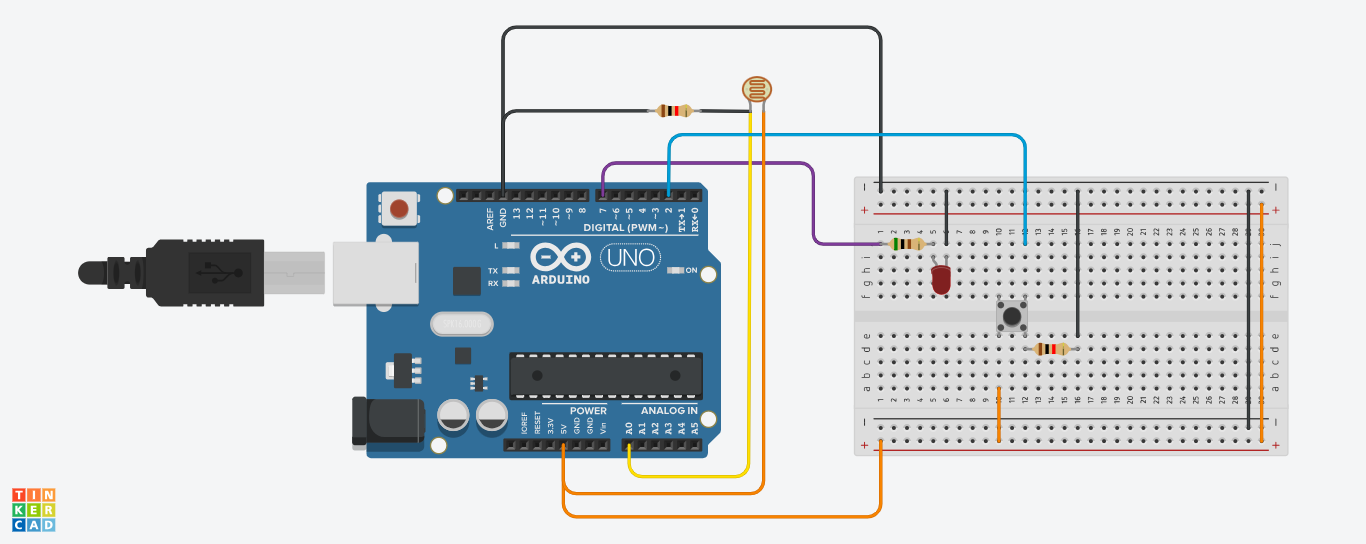
\includegraphics[width=1\linewidth]{img/Tinkercad.png}
    \caption{Triển khai mạch ESP32 trên Wokwi}
    \label{fig:tinkercad}
\end{figure}

Hệ thống được giả lập trên \href{https://wokwi.com/projects/418228728977255425}{Wokwi} được mô tả như hình~\ref{fig:tinkercad} này sử dụng ESP32 và bao gồm các thành phần: cảm biến ánh sáng (LDR), đèn LED và nút nhấn. Cảm biến ánh sáng được kết nối với cổng esp:35 của ESP32 thông qua một điện trở cho phép ESP32 đo mức điện áp thay đổi theo cường độ ánh sáng xung quanh. Đèn LED được điều khiển thông qua cổng esp:14 của ESP32, có thể phản hồi lại theo tín hiệu từ cảm biến ánh sáng hoặc tín hiệu từ nút nhấn. Nút nhấn cho phép người dùng chuyển chế độ vận hành hệ thống từ AutoMode sang ManualMode và điều khiển đèn LED bật/tắt một cách thủ công. Thông qua đó ta thấy hệ thống phiên bản giả lập trên Wokwi giải quyết tương đối đầy đủ những yêu cầu mà đặc tả và bản thiết kế hệ thống đã đề ra. Ngoài ra, người dùng có thể kết nối với WiFi giả lập của Wokwi để kết nối MQTT và truyền dữ liệu lên Internet.  


\pagebreak
\subsection{Triển khai hệ thống trên thiết bị thật}
\begin{figure}[H]
    \centering
    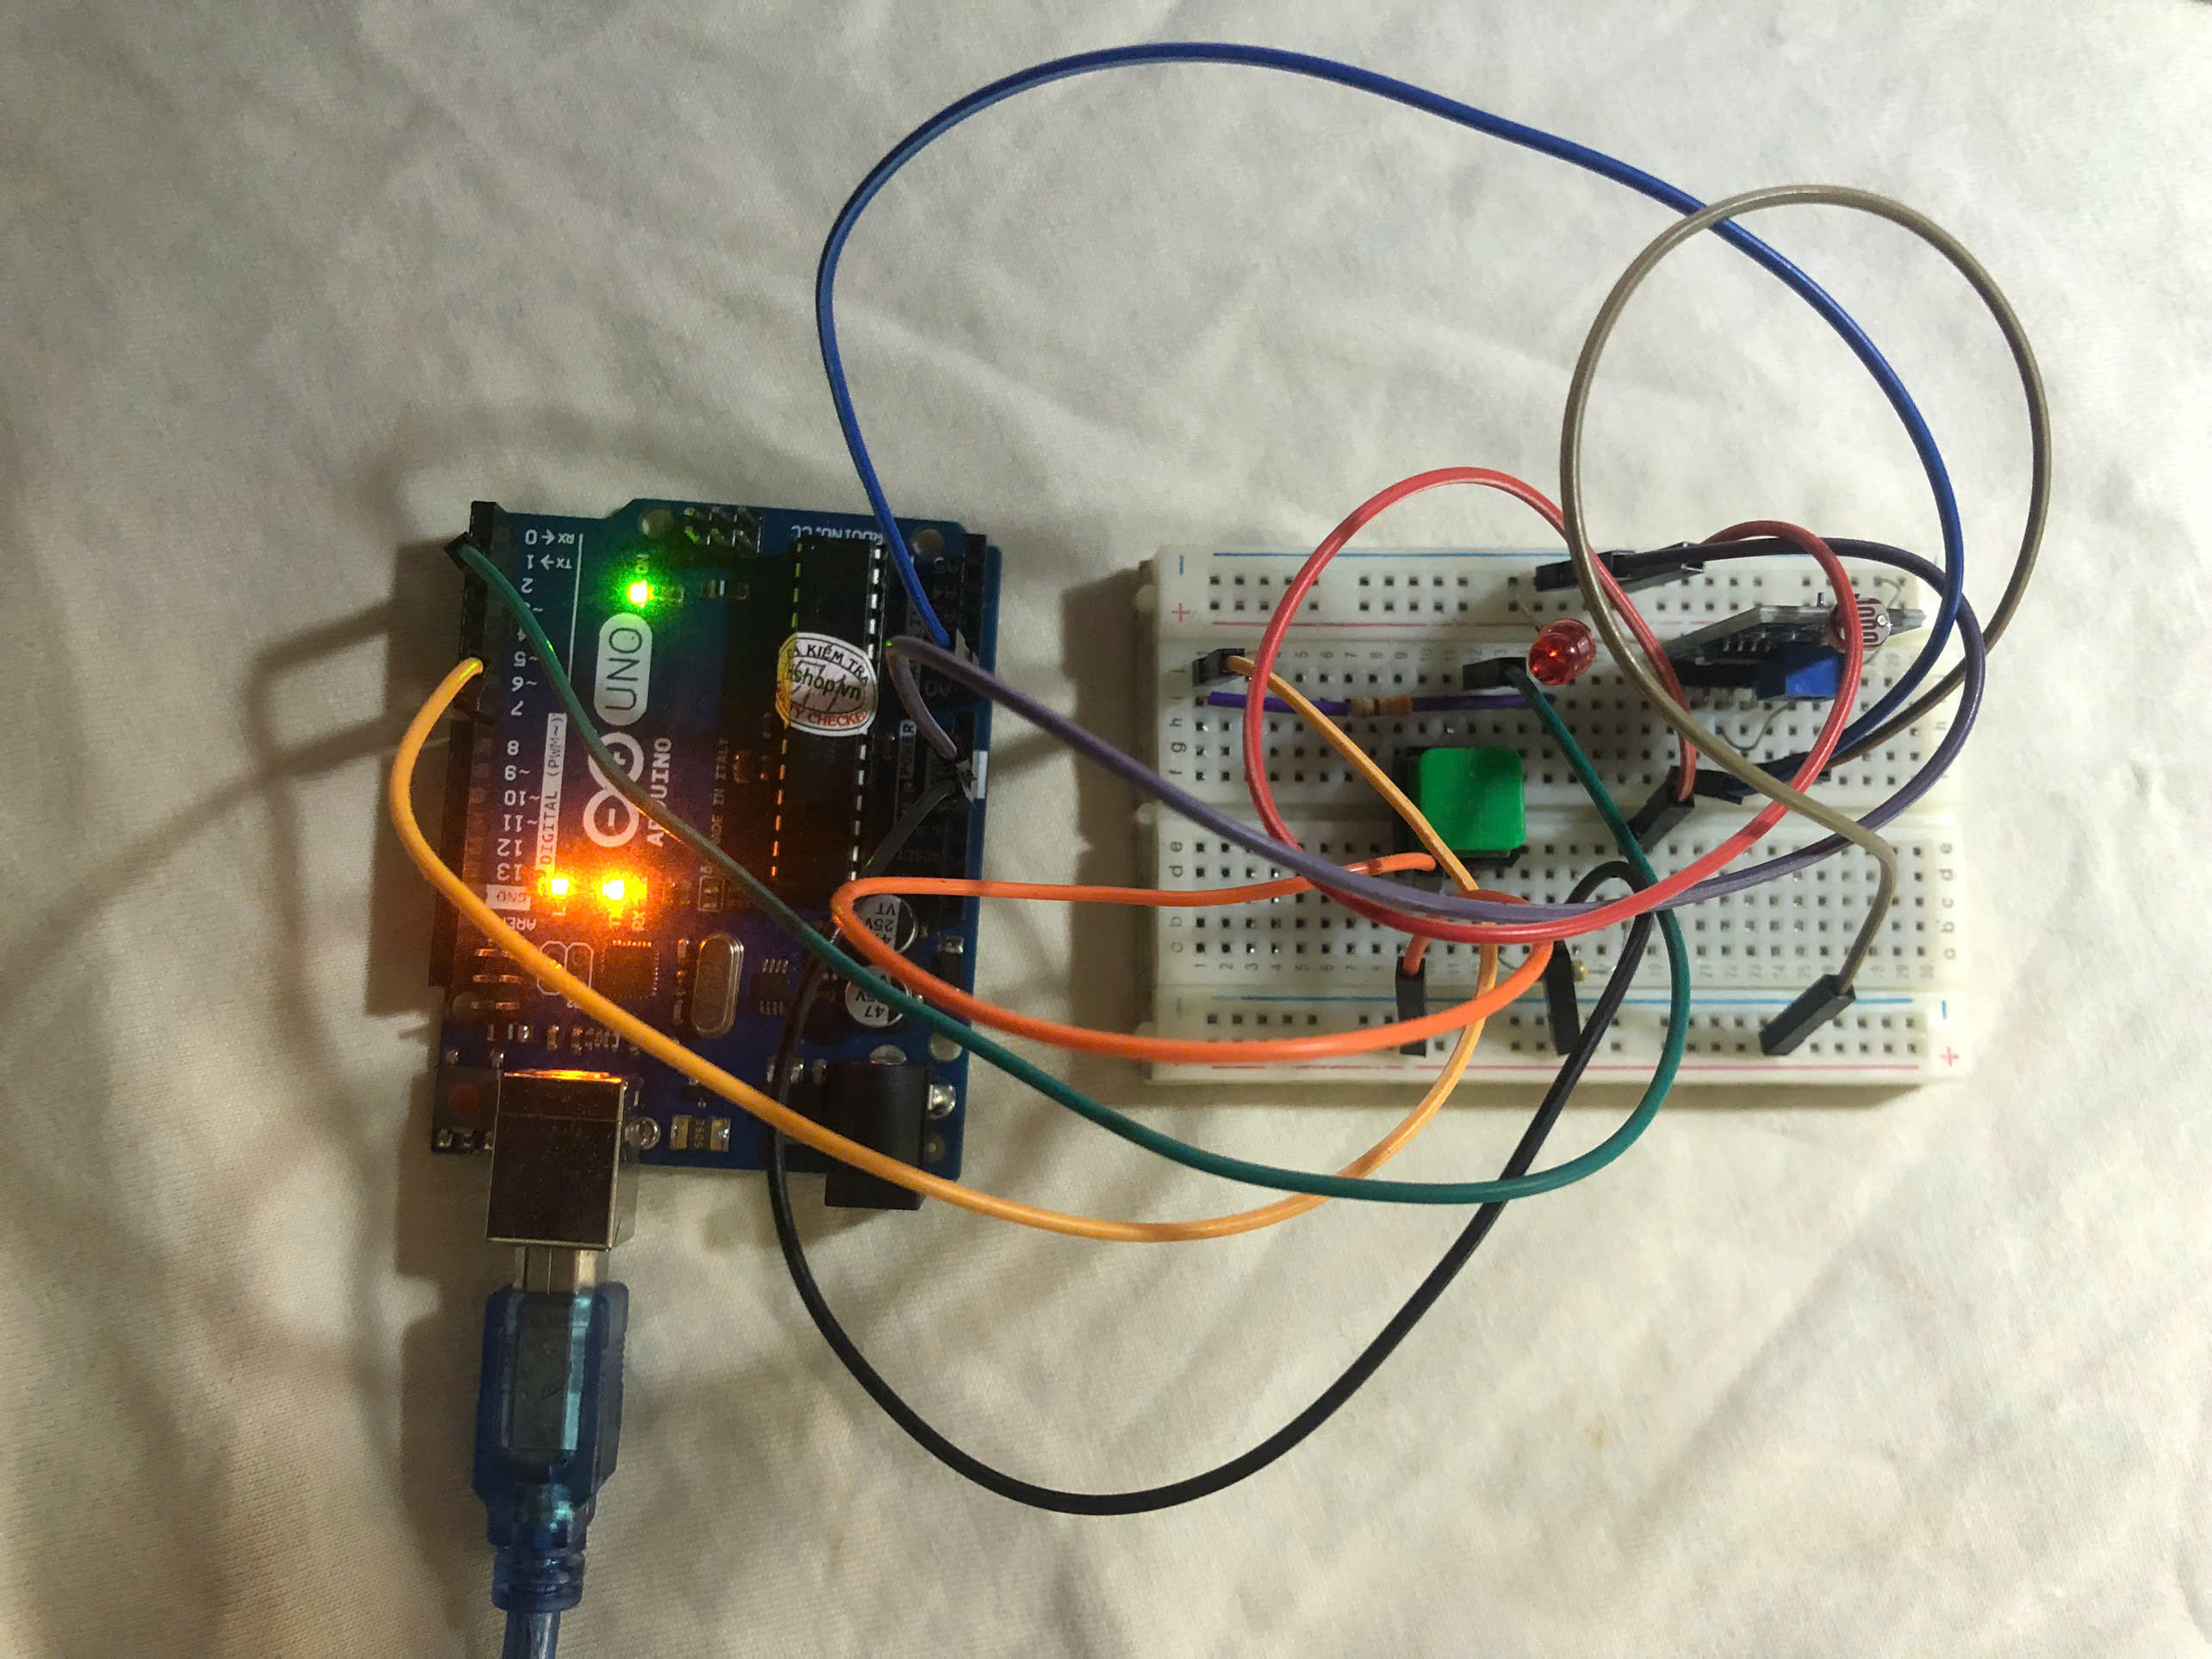
\includegraphics[width=\textwidth]{img/realSystem.jpg}
    \caption{Triển khai hệ thống thực tế}
    \label{fig:real_1}
\end{figure}


Hệ thống thực tế trên hình~\ref{fig:real_1} được bố trí và lắp đặt tương tự như triển khai giả lập trên Wokwi ở hình~\ref{fig:tinkercad}. Mạch được cung cấp nguồn và nạp code bằng USB Port nối với Laptop và sẽ truyền nhận dữ liệu giữa mạch và Laptop thông qua kết nối không dây WiFi đến MQTT. 


\pagebreak
\subsection{Giới thiệu chức năng website}
Website gồm có các chức năng sau: 
\begin{itemize}
    \item Theo dõi trạng thái đèn bao gồm Off, On và Blinking.
    \item Theo dõi chế độ vận hành hệ thống hiện tại (Auto Mode hay Manual Mode thông qua màu sắc của Delay Duration), trạng thái ánh sáng môi trường xung quanh hệ thống (Day hay Night thông qua màu sắc của Light Sensor), timeout từ Manual Mode sang Auto Mode bao nhiêu Millisecond (nếu hiển thị 0 thì hệ thống sẽ bỏ qua điều kiện timeout này khi vận hành)
    \item Người dùng có thể dùng lệnh (bằng text hoặc voice) để điều khiển hệ thống từ xa, thông qua giao tiếp MQTT, truyền dữ liệu kết nối không dây WiFi và LLMs (Generative AI) để phân tích yêu cầu người dùng.
\end{itemize}


\begin{figure}[H]
    \centering
    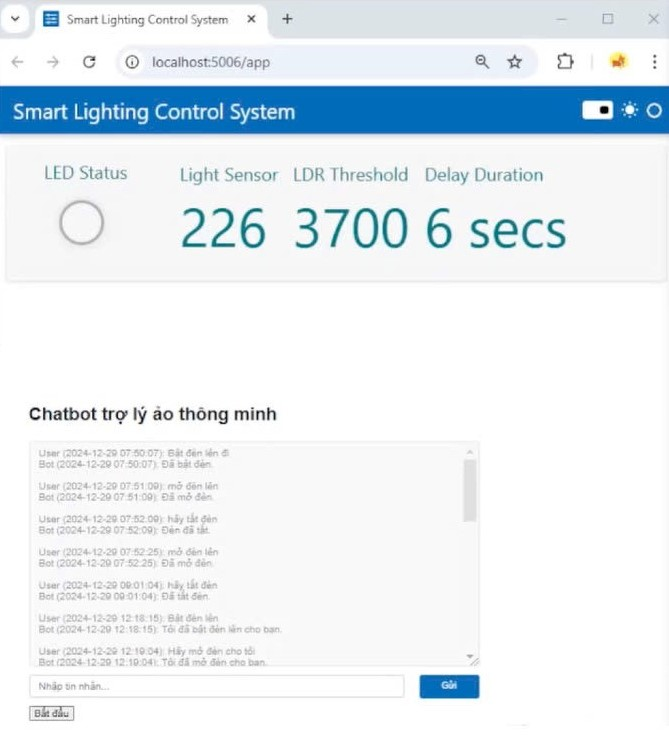
\includegraphics[width=0.6\textwidth]{img/UI.jpg}
    \caption{Giao diện website}
    \label{fig:website}
\end{figure}

\begin{figure}[H]
    \centering
    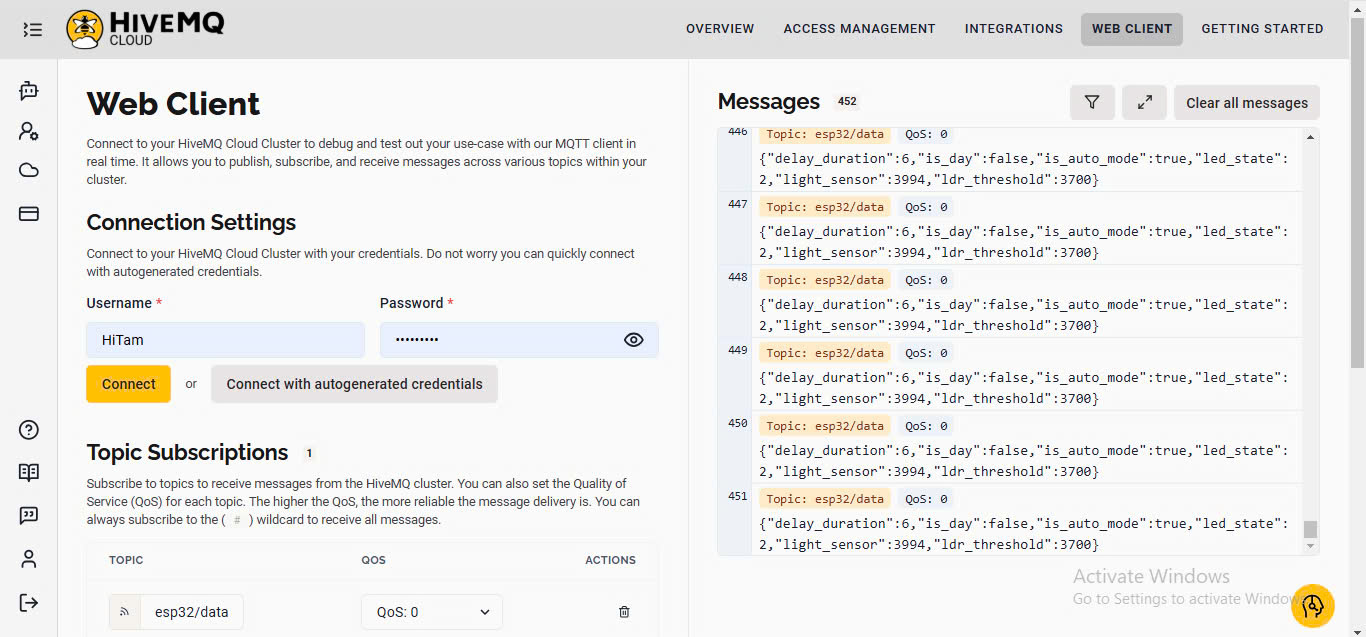
\includegraphics[width=\textwidth]{img/MQTT.jpg}
    \caption{Giao diện trang web theo dõi MQTT}
    \label{fig:mqtt}
\end{figure}

\begin{figure}[H]
    \centering
    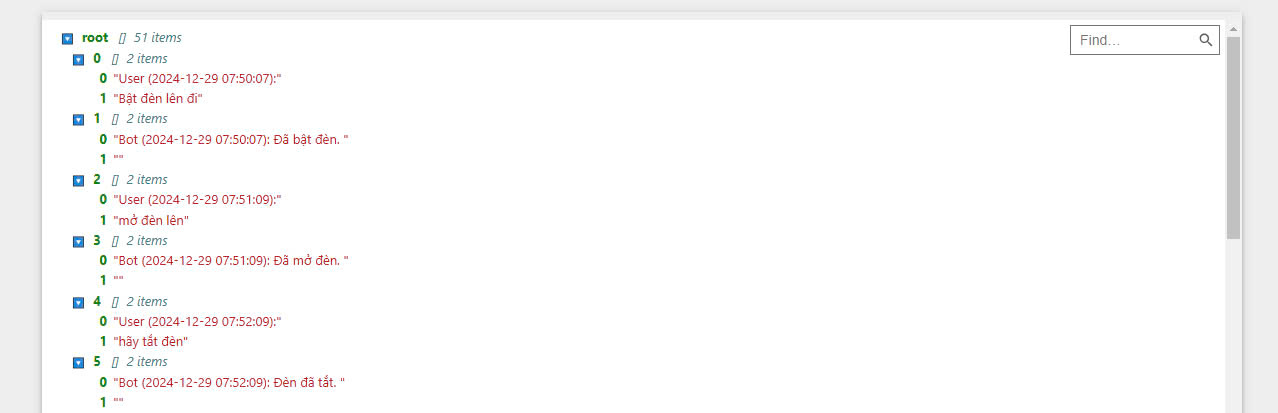
\includegraphics[width=\textwidth]{img/chat-history.jpg}
    \caption{Cấu trúc JSON lưu trữ lịch sử nhắn tin}
    \label{fig:mqtt}
\end{figure}

\pagebreak
\subsection{Release}
\begin{lstlisting}[escapeinside={(*@}{@*)}]
21127423,Tran Hieu Tam,(*@\href{https://youtube.com/playlist?list=PL49PFd0rcrSMamwSboGjRe7nyyKdWxkfa&feature=shared}{https://youtube.com/playlist?list=PL49PFd0rcrSMamwSboGjRe7nyyKdWxkfa&feature=shared}@*),(*@\href{https://drive.google.com/drive/folders/1Dzda6UcX8GyJiqW1w3eEMZk_fvy09f99?usp=sharing}{https://drive.google.com/drive/folders/1Dzda6UcX8GyJiqW1w3eEMZk_fvy09f99?usp=sharing}@*)
\end{lstlisting}

% Author: Trần Hiếu Tâm

% Contact email: \href{thtam21@clc.fitus.edu.vn}{thtam21@clc.fitus.edu.vn}

% Release date: November 11th, 2024

% Release version: 1.0

% Location: Ho Chi Minh City, Viet Nam

% Copyright: Faculty of Information Technology, VNUHCM - University of Science

% GitHub repository: \href{https://github.com/HieuTam/HCMUS-IoT-SmartLightingControlSystem}{https://github.com/HieuTam/HCMUS-IoT-SmartLightingControlSystem}


\vspace{1cm}
{\small
\subsubsection*{Project Information}

\begin{itemize}
    \item \textbf{Release Version:} 1.0
    \item \textbf{Release Date:} December 30, 2024
    \item \textbf{Author:} Trần Hiếu Tâm
    \item \textbf{Contact Email:} \href{mailto:thtam21@clc.fitus.edu.vn}{thtam21@clc.fitus.edu.vn}
    \item \textbf{Location:} Ho Chi Minh City, Viet Nam
    \item \textbf{GitHub Repository:} \href{https://github.com/HieuTam/HCMUS-IoT-SmartLightingControlSystem}{https://github.com/HieuTam/HCMUS-IoT-SmartLightingControlSystem}\\[1cm]
\end{itemize}

\subsubsection*{Copyright}
\noindent Faculty of Information Technology, VNUHCM-University of Science
}\\[1.5cm]

\begin{figure}[H]
    \centering
    
\includegraphics[width=0.35\linewidth]{img/Logo-HCMUS-Symbol.png}
\end{figure}

% References
\cleardoublepage
\phantomsection
\addcontentsline{toc}{section}{Tài liệu tham khảo}
\bibliographystyle{plain}
\nocite{*} % Includes all references from the .bib file
\bibliography{ref/ref}


% Appendix
% \appendix
% Add \cleardoublepage to move appendices to next page.
% \section{Phụ lục}
\begin{itemize}
\item Template này \textbf{không phải} là template chính thức của Khoa Công nghệ thông tin - Trường Đại học Khoa học Tự nhiên.
\item Các hình ảnh, bảng biểu, thuật toán trong template chỉ mang tính chất ví dụ.
\item Nhóm tác giả phân phối \textbf{miễn phí} template này \href{https://github.com/khongsomeo/hcmus-unofficial-report-template}{trên GitHub} và \href{https://www.overleaf.com/latex/templates/hcmus-report-template/zyrhmsxynwqs}{trên Overleaf} với \href{https://github.com/khongsomeo/hcmus-unofficial-report-template/blob/main/LICENSE}{Giấy phép GNU General Public License v3.0}. Nhóm tác giả không chịu trách nhiệm với các bản phân phối không nằm trong hai kênh phân phối chính thức nêu trên.
\end{itemize}

\end{document}